\chapter{Agrupamento de séries temporais} \label{cap:agrupamento_series_temporais}

Por agrupamento, entende-se a tarefa de dividir um conjunto de dados em grupos homogêneos e bem definidos. A partir de determinada métrica de dissimilaridade, o agrupamento busca formar grupos que contêm dados que possuem baixa dissimilaridade entre si, ao passo que estes possuem alta dissimilaridade com os dados contidos nos demais grupos. O agrupamento se faz necessário quando não se possui, \emph{a priori}, a rotulação dos dados, ou seja, não se sabe a qual grupo cada instância pertence, e em alguns casos, não se sabe até mesmo o número de grupos que as instâncias estão naturalmente contidas. A partir da realização de tal tarefa, espera-se adquirir conhecimento acerca da estrutura dos dados bem como extrair informação útil dos mesmos.

O agrupamento pode ser feito em dados textuais, categóricos, binários, numéricos, ordinais, relacionais, temporais, espaço-temporais, ou qualquer combinação destes. Quando o agrupamento é realizado em dados nos quais a observação das grandezas de interesse não variam com o tempo, os dados são considerados estáticos, e caso contrário os dados são ditos dinâmicos. As séries temporais, que são objeto de estudo deste trabalho, são dados dinâmicos. Grande parte da pesquisa de agrupamento se dá na análise de dados estáticos, no entanto, existe uma tendência de crescimento no estudo em séries temporais devido às diversas aplicações nas engenharias, mercado financeiro, marketing, medicina, biologia, meteorologia, astronomia entre outros ~\parencite{Liao}.

Formalmente, uma partição $\mathcal{C}$ é a partição de um conjunto de dados $X$ composto por $n$ instâncias, e cada instância possuindo $d$ características, em $k$ sub-conjuntos mutualmente disjuntos, $\mathcal{C}_1,\mathcal{C}_2,...,\mathcal{C}_k$. A esses sub-conjuntos dá-se o nome de grupos. Dessa maneira,

\begin{equation}
\mathcal{C} = {\mathcal{C}_1,\mathcal{C}_2,...,\mathcal{C}_k} \text{,  tal que } \mathcal{C}_k \cap \mathcal{C}_l = \emptyset
\end{equation}

Uma série temporal é definida como um conjunto de observações sequenciais de uma grandeza de interesse, assim, ela é um tipo de dados com valores reais e de alta dimensionalidade. Denomina-se de tamanho da série temporal o número de observações ou amostras que ela contém.

As seções a seguir deste capítulo descrevem as principais estratégias de agrupamento de séries temporais. Por estratégia entende-se a escolha de:
\begin{itemize}
	\item um pré-processamento dos dados (normalização),
	\item uma métrica de dissimilaridade para se comparar as instâncias,
	\item um algoritmo de agrupamento para a realização do agrupamento em si,
	\item e, finalmente, um índice de validação para avaliar a qualidade da partição resultante.
\end{itemize}
Este capítulo se encontra estruturado de forma a realizar um estudo de cada um destes aspectos. Inicialmente, na primeira seção, são analisadas as opções de pré-processamento dos dados, que consistem, basicamente em normalizar, e reduzir o tamanho das séries temporais.

 Em seguida, são analisadas as métricas de dissimilaridade de séries temporais que podem ser divididas em: métricas baseadas em distâncias ou dissimilaridades, aplicadas no espectro das séries temporais e em modelos estatísticos ~\parencite{Liao}. Pelo fato da escolha de uma métrica de dissimilaridade ser um dos aspectos centrais na tarefa de agrupamento  de séries temporais as principais métricas apresentadas na literatura são discutidas na maior parte deste capítulo.
 
 A escolha da métrica de dissimilaridade se dá pela definição de um critério, ou métrica , que nos diga o quão similares duas instâncias são. Tal métrica é dependente do objetivo principal da tarefa de agrupamento. Existem determinadas aplicações que realizam o agrupamento baseado no valor da predição da série temporal, ou seja, as curvas são agrupadas em função do próximo valor esperado de cada série, enquanto em outras aplicações, quando se deseja comparar o formato das séries, o uso de métricas ponto a ponto se adequa melhor. Existem ainda outras abordagens que buscam agrupar curvas que possuam o mesmo comportamento ou tendência, ou seja, curvas que se mantêm constante, aumentam ou diminuem o seu valor em períodos de tempo próximos.

Após a discussão das métricas, serão expostos os principais algoritmos de agrupamento de séries temporais disponíveis na literatura. Estes algoritmos podem ser estocásticos como o \emph{k-means}, \emph{k-medoids}, ou de agrupamento hierárquico com diferentes tipos de \emph{linkagem}, tais como: a \emph{average}, \emph{complete} ou \emph{ward}. Existem também os algoritmos de agrupamento baseados em densidade, como o \emph{DBSCAN}, que possuem a vantagem de, não ser necessária a definição, \emph{a priori}, do número de grupos.

Finalmente, na última seção do capítulo, são apresentados os principais índices de validação de agrupamentos disponíveis na literatura. Tais índices são essenciais para se mensurar a qualidade das partições dos dados resultantes dos algoritmos de agrupamento.

Tal revisão bibliográfica é importante para a definição da melhor estratégia, ou seja, da escolha de uma normalização, métrica de dissimilaridade, algoritmo de agrupamento e índice de validação das partições resultantes a ser empregada no agrupamento das curvas de carga.

\section{Pré-processamento de séries temporais}

Antes da tarefa de agrupamento em si, recomenda-se a realização de uma fase de pré-processamento dos dados, nos quais eles são normalizados. A normalização é utilizada para corrigir possíveis distorções que o dados brutos podem apresentar devido ao seu processo de aquisição. Pode-se corrigir distorções relacionadas à escala, translação, rotação, diferença de fase, entre outras.

Além da normalização, métricas de dissimilaridade podem ser aplicadas no espectro das séries temporais, como uma estratégia de redução de dimensionalidade, para a posterior realização da tarefa de agrupamento. Tal redução é desejada, pela ocorrência do "mal da dimensionalidade", que basicamente nos diz que quando o número de dimensões de cada instância de um conjunto de dados é muito grande, as instâncias tendem a se encontrar espaçadas e equidistantes, fazendo com que seja necessário um número muito grande de instâncias para a construção de uma fronteira de decisão ~\parencite{DudaHart}. Dessa maneira, faz-se necessária um etapa de pré-processamento, e as principais abordagens se encontram detalhadas a seguir.

\subsection{Normalização} \label{sec:norm_Z}

Estudos demonstram que qualquer tarefa de mineração de dados de séries temporais sem algum tipo de normalização é sem sentido ~\parencite{Keogh_need_norm}. O tipo de normalização mais comum no contexto de séries temporais é realizado por meio da normalização Z ~\parencite{trillions}, na qual, e média $\mu$ e o desvio padrão $\sigma$ de cada série temporal de tamanho $n$ é calculada e é feita a seguinte transformação em cada medição da série $\bf{x}$

\begin{equation}
\hat{x_i} = \frac{x_i - \mu}{\sigma}, i = 1,...,n.
\end{equation}

No contexto de séries temporais, a normalização Z é extremamente importante para remover certas imperfeições e diferenças de escala que surgem a partir da geração das séries temporais, sejam estas obtidas por meio de medições ou de algum tipo de transformação de dados. Na figura ~\ref{fig:z_norm} podem ser vistas duas senoides, $s1$ e $s2$, ligeiramente defasadas mas com diferença significativa em amplitude e valor médio, ou \emph{offset}. Na mesma figura, as suas respectivas versões normalizadas podem ser vistas pelas linhas tracejadas. É notável que as curvas tracejadas são bem mais semelhantes entre si, e caso as diferenças de amplitude e valor médio não sejam relevantes para a tarefa de agrupamento ou classificação, o que é geralmente o caso, então a normalização Z é uma etapa de pré-processamento recomendada.
\begin{figure}[h!]
	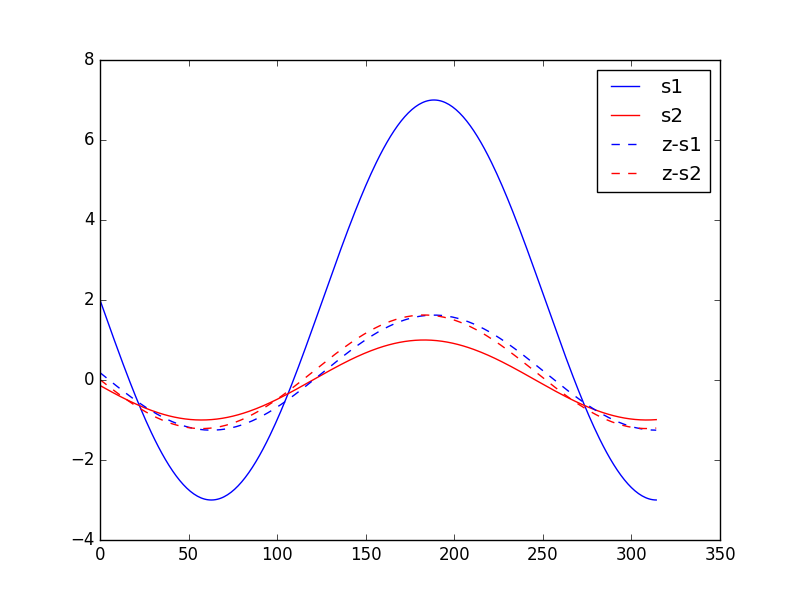
\includegraphics[width=\linewidth]{figuras/z_norm.png}
	\caption{Exemplo de normalização Z. As duas senóides s1 e s2 que possuem comportamento semelhante mas, devido à diferença de \emph{offsets} e  amplitudes, se apresentam significativamente distintas. Após a aplicação da normalização Z em cada uma delas (z-s1 e z-s2), elas são praticamente idênticas, }
	\label{fig:z_norm}
\end{figure}
 Em ~\parencite{trillions} é mencionado que em tarefas de classificação com séries temporais não normalizadas e Z-normalizadas, obteve-se uma taxa de erro 50\% maior no primeiro caso em relação ao segundo quando é inserido um \emph{offset} de apenas $\pm$5\%.
 
Além da normalização Z, podem ser utilizadas também as normalizações max e min-max, nas quais devem ser aplicadas, respectivamente, as seguintes transformações em cada uma das $n$ medições da série $\bf{x}$:

\begin{equation}
\hat{x_i} = \frac{x_i}{\max(\bf{x})}, i = 1,...,n \text{          e}
\end{equation}

\begin{equation}
\hat{x_i} = \frac{x_i-\min(\bf{x})}{\max(\bf{x}) - \min(\bf{x})},  = 1,...,n.
\end{equation}

A primeira é utilizada, em geral, quando os valores observados das séries temporais que compõem o conjunto de dados são sempre positivas, e confina a série no intervalo $[0,1]$ dividindo cada valor pelo maior valor observado em toda série. Já a segunda, também confina a série no intervalo $[0,1]$, mas necessariamente seu menor valor se torna $0$, o que nem sempre ocorre na primeira. Os efeitos de ambas normalizações podem ser vistos na figura ~\ref{fig:norms}. Como os valores de medição dos medidores inteligentes são sempre positivos, a normalização max é muito utilizada na mineração de dados de Redes Elétricas Inteligentes ~\parencite{Chicco}.
\textbf{}
\begin{figure}[h!]
	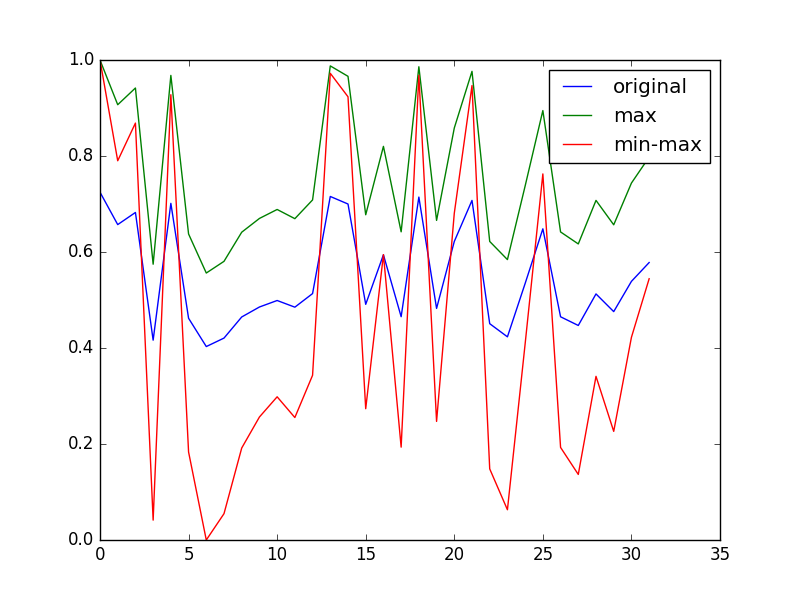
\includegraphics[width=\linewidth]{figuras/normalizations.png}
	\caption{Exemplos de normalização max e min-max.}
	\label{fig:norms}
\end{figure}

\subsection{\emph{Piecewise aggregate approximation} - 
	PAA}

A \emph{Piecewise aggregate approximation} é uma técnica de redução de dimensionalidade na qual, basicamente, a série temporal é dividida em $w$ janelas de tamanhos iguais e o valor da série neste intervalo é definido como o valor médio da série no intervalo compreendido pela janela ~\parencite{SAX}. Assim, dada uma série temporal $\bm{x} = x_1,x_2,...,x_n$ de tamanho $n$, esta pode ser representada em  um espaço $w$ dimensional, sendo $w<n$ e $w$ múltiplo inteiro de $n$, por um vetor $\bm{\bar{x}} =\bar{x_1},\bar{x_2},...,\bar{x_w} $, tal que seu $i$-ésimo elemento é dado por

\begin{equation}
	\bar{x_i} = \frac{w}{n} \sum_{j=\frac{n}{w}(i-1)+1}^{\frac{n}{w}i} x_j.
\end{equation}
%\begin{equation}
%	\bar{x_i} = \frac{w}{n} \mathop{\mathlarger{\mathlarger{\mathlarger{\mathlarger{\sum}}}}}_{j=\frac{n}{w}(i-1)+1}^{\frac{n}{w}i} x_j.
%\end{equation}
Na figura \ref{fig:PAA} pode ser vista a redução de dimensionalidade da senoide em azul formada por 315 pontos para a curva em vermelho, formada por 19 pontos. Em ~\parencite{fuzzy_transform} é sugerida uma técnica de redução de dimensionalidade de séries temporais que pode ser vista como uma versão fuzzy da PAA. Basicamente, a ideia é definir uma partição fuzzy para o espaço de entrada e definir um coeficiente para cada valor da partição.

\begin{figure}[h!]
	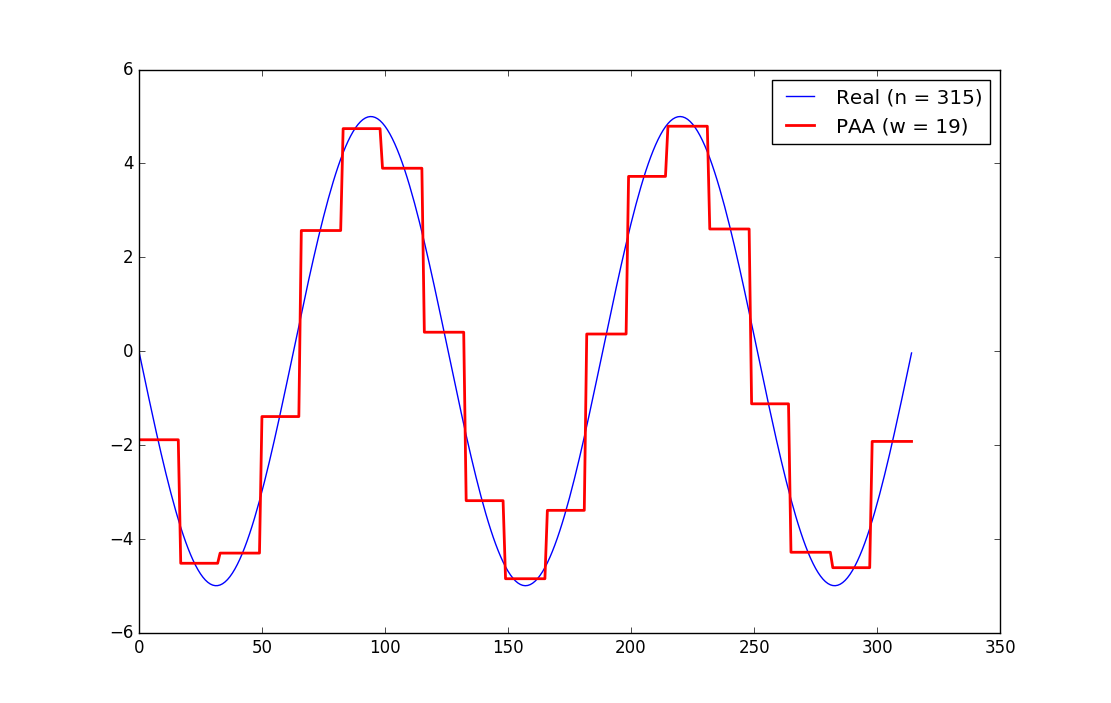
\includegraphics[width=\linewidth]{figuras/PAA.png}
	\caption{Exemplo de redução de dimensionalidade pela PAA.}
	\label{fig:PAA}
\end{figure}




%\subsubsection{Symbolic Aggregate Approximation - SAX}


%\hl{TODO...}

\subsection{Transformada discreta de Fourier - DFT}

Ao se calcular a série de Fourier para os vetores $\bm{x}$ e $\bm{y}$, a distância entre os dois vetores pode ser obtida pelo cálculo de qualquer umas das métricas de distância a serem discutidas, como a distância euclidiana, entre os coeficientes da série de Fourier discreta truncada de cada vetor 

\begin{equation}
dist(\bm{x},\bm{y}) = \bigg(\sum_{i=1}^{\theta} (\hat{x_i} -\hat{y_i})^2 \bigg)^{\frac{1}{2}},
\end{equation}
onde $\theta$ é o número de coeficientes complexos a serem utilizados, e $\hat{x_i}$ e $\hat{y_i}$ são os i-ésimos termos da transformada discreta de Fourier, ou \emph{Discrete Fourier Transform} (DFT), dos vetores $\bm{x}$ e $\bm{y}$ respectivamente.

Segundo ~\parencite{FFT}, são necessários apenas 5 coeficientes ou menos para uma boa aproximação das curvas no domínio da frequência, e a distância euclidiana no domínio da frequência é análoga à distância euclidiana no domínio do tempo pelo teorema de \emph{Parseval}, sendo, portanto, a métrica de distância mais indicada.

O método proposto tem a vantagem de realizar uma redução significativa de dimensionalidade, já que uma série temporal com 300 pontos, por exemplo, pode ser reduzida para uma análise em 5 pontos. Além disso, quando existe a presença de ruídos de alta frequência no sinal, e tais ruídos não são relevantes para o agrupamento, tal abordagem acarreta em resultados melhores.

%\subsubsection{Transformada discreta \emph{Wavelet} - DWT}

%\hl{TODO: Completar...}

%\subsubsection{Decomposição em valores singulares - SVD}

%A decomposição em valores singulares (\emph{Singular Value Decomposition}), ou SVD, é uma estratégia de redução de dimensionalidade dos dados baseada na obtenção dos autovalores e autovetores da matriz que contém os dados.  Segundo ~\parencite{Ullman}, a vantagem da SVD é a representação de conceitos que se encontram ocultos na matriz de dados originais.

%Assim, dada uma matriz $M_{nxd}$ contendo os dados, onde $n$ é o número de instâncias e $d$ é o número de dimensões das instâncias, ela pode ser decomposta em:

%\begin{equation}
%M = U \Sigma V^T,
%\end{equation}
%onde $U$ é a matriz dos autovetores de $MM^T$, enquanto $V$ e $\Sigma$ são respectivamente a matriz dos autovetores e a matriz diagonal contendo a raiz quadrada dos autovalores de $M^{T}M$.

%A diagonal da matriz $\Sigma$ deve ser formada pelos autovalores de forma ordenada, em função do seu valor absoluto, e a i-ésima coluna da matriz $V$ deverá ser o autovetor associado ao autovalor contido na i-ésima coluna da matriz $\Sigma$. Os autovalores são sempre positivos e a eles dá-se o nome de valores singulares. Assim temos, 

%\[
%\Sigma=
%\begin{bmatrix}
%\lambda_1 & 0 & ... & 0 \\
%0 & \lambda_2 & ... & 0 \\
%0 & 0 & ... & 0 \\
%0 & 0 & ... & \lambda_n 
%\end{bmatrix} \quad
%\text{e, }
%V=
%\begin{bmatrix}
%e_{1_1} & e_{2_1} & ... & e_{n_1} \\
%e_{1_2} & e_{2_2} & ... & e_{n_2} \\
%e_{1_3} & e_{2_3} & ... & e_{n_3} \\
%e_{1_4} & e_{2_4} & ... & e_{n_4} 
%\end{bmatrix}\text{,}
%\]
%onde o autovalor $\lambda_i$ está associado ao autovetor $e_i$, e $\lambda_1 \geq \lambda_2 \geq ...\geq\lambda_n > 0$.

%Caso os primeiros elementos da diagonal da matriz $\Sigma$ sejam muito maiores que os últimos elementos, então a matriz de dados $M$ pode ser reduzida para um número $r$ de dimensões, sendo $r<d$, de maneira a tornar mais claros os conceitos ocultos nos dados.

%Segundo ~\parencite{Ullman} Uma boa maneira de se escolher o número $r$, é reter os primeiros autovalores cujo a soma dos seus quadrados corresponde a pelo menos $90\%$ da soma total dos quadrados de todos os autovalores da matriz $\Sigma$. Assim, a matriz reduzida, e que representa os dados, $M_{nxr}^{'}$, é obtida por:

%\begin{equation}
%M_{nxr}^{'} = MV_{r}^{T},
%\end{equation}
%onde $V_{r}^{T}$ é a matriz $V$ somente com os seus $r$ primeiros autovetores  associados.

%Neste momento vale destacar que a decomposição em valores singulares é uma técnica de redução de dimensionalidade que é aplicada em todo o conjunto de dados, ao passo que técnicas como DFT e DWT são aplicadas a cada instância. \hl{TODO: Comentar acerca do custo computacional}


\section{Métricas de dissimilaridade} \label{sec:metricas}

Existem diversas métricas de dissimilaridade para comparar duas séries temporais, e elas divergem entre si principalmente no que diz respeito aos custos computacionais, sensibilidade à ruídos, invariância ao defasamento entre as curvas, capacidade de ser utilizada para séries temporais com diferentes tamanhos, entre outros. Além disso, as métricas podem ser divididas em dois grandes grupos, sendo o primeiro formado pelas métricas que podem ser consideradas distâncias, e aquelas que não podem. Para determinada métrica ser considerada uma distância ela deve possuir, necessariamente, as seguintes propriedades para vetores $\bm{x},\bm{y}$ e $\bm{z}$ ~\parencite{DudaHart}:

%DudaHart-pg 31

\begin{itemize}
	\item não-negatividade:
	\begin{equation}
	dist(\bm{x},\bm{y}) > 0, \forall \text{ }  \bm{x},\bm{y} \in \mathbb{R}^{n}\text{,}
	\end{equation}
	\item reflexividade:
	\begin{equation}
	dist(\bm{x},\bm{y}) = 0\text{, se, e somente se, }\bm{x}=\bm{y}\text{,}
	\end{equation}
	\item simetria:
	\begin{equation}
	dist(\bm{x},\bm{y}) = dist(\bm{y},\bm{x})\text{,}
	\end{equation}
	\item desigualdade do triângulo:
	\begin{equation}
	dist(\bm{x},\bm{z}) + dist(\bm{z},\bm{y}) \geq dist(\bm{x},\bm{y}).
	\end{equation}
\end{itemize}

Nas subseções seguintes desta seção, encontram-se algumas métricas que atendem à todas ou à algumas dessas propriedades e que serão detalhadas em cada uma das características já expostas e esperadas de uma métrica de similaridade entre duas séries temporais. Ao fim do capítulo se encontra a Tabela ~\ref{tbl:dissimlarity_summary_table} que sumariza todas  as informações discutidas nesta seção. 

Vale mencionar, neste momento, que existem métricas de dissimilaridade obtidas por meio de modelos estatísticos das séries temporais que sejam representativos de cada uma das séries temporais a serem comparadas. Supõe-se que elas foram geradas por modelos paramétricos, sendo o modelo ARIMA um dos modelos mais utilizados. A obtenção da medida de dissimilaridade entre as séries se dá a partir da comparação entre os parâmetros desses modelos. As métricas obtidas a partir de modelos estatísticos possuem aplicação maior em agrupamentos de séries temporais baseados na predição delas, não sendo assim, em geral, aplicáveis à problemas de agrupamento de curvas de carga, e por isso não serão abordadas nesta dissertação de mestrado. No entanto, algumas das abordagens neste sentido, assim como outras referências, podem ser encontradas em ~\parencite{TSCLUST}.

\subsection{Minkowski}

A distância de Minkowski é definida como
\begin{equation}
dist(\bm{x},\bm{y}) = \bigg (\sum_{i}^{n} |x_i -y_i|^p \bigg)^{\frac{1}{p}}.
\end{equation}

A métrica de Minkowski é também conhecida como norma $L_p$, e tem como casos notáveis a distância Euclidiana, ou $L_2$, quando $p=2$, a distância \emph{Manhattan}, ou $L_1$, quando $p=1$ e a distância \emph{Chebyshev}, ou $L_\infty$, quando $p\to\infty$.

\begin{figure}[h!]
	  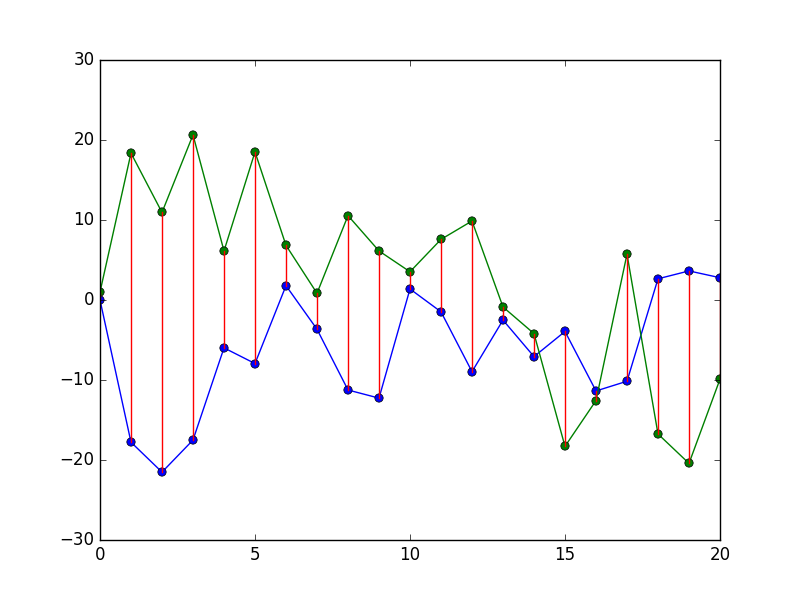
\includegraphics[width=\linewidth]{figuras/dist_euclidiana.png}
	  \caption{Distância Euclidiana entre as duas curvas é dada pela soma das distâncias euclidianas entre as observações de cada curva no mesmo instante.}
	  \label{fig:dist_euclidiana}
\end{figure}

Na figura ~\ref{fig:dist_euclidiana} encontram-se duas séries temporais, na tabela ~\ref{minkowski_table} os valores de distância obtidos variando-se o valor de $p$. Pela tabela, pode-se notar que pequenas variações no valor de $p$ acarretam em grandes variações no valor da métrica, bem como que este valor diminui ao passo que $p$ aumenta.A métrica de Minkowski atende à todas as propriedades das métricas de distância e, dessa maneira, pode ser considerada uma distância, e o seu custo computacional é $\mathcal{O}(n)$, onde $n$ é o número de amostras ou observações das séries a serem comparadas.


\begin{table}[!h]
	\centering
	\caption{Distâncias Minkowski entre as curvas da figura ~\ref{fig:dist_euclidiana} para diversos valores de $p$.}
	\label{minkowski_table}
	\begin{tabular}{|c|c|c|c|c|c|c|}
		\hline
	%	\toprule
			%\begin{tabular}{llllllll}
						& p=1    & p=2   & p=3   & p=4 &p=5 & p$\to \infty$ \\ \hline
%		\midrule
		distância & 318.18 & 86.88 & 59.59 & 50.54 & 44.03 & 38.14   \\ \hline
	%	\bottomrule
	\end{tabular}
\end{table}


\subsection{\emph{Dynamic Time Warping} - DTW}

A \emph{Dynamic Time Warping} é, talvez, a métrica de dissimilaridade mais utilizada para dados de séries temporais. Proposta inicialmente para ser utilizada em problemas de detecção de fala, a DTW se mostrou útil para tarefas de mineração de dados em séries temporais ~\parencite{DTW}.

Dada duas séries temporais $\bm{x} = x_1,x_1,x_3,...,x_i,...,x_n$ e $\bm{y} = y_1,y_2,y_3,...,y_j,...,y_m$, suponha que seja feito a construção de um \emph{grid} $n_{x}m$, no qual na posição $(i,j)$ se encontra o valor resultante de uma métrica de distância $\delta(i,j)$ entre os pontos $x_i$ e $y_j$. Tal métrica pode ser, por exemplo, a já citada distância Minkowski. A partir deste \emph{grid}, é construído um caminho $W=w_1,w_2,w_3,...,w_k$, onde cada $w_k$ corresponde à alguma posição $(i,j)_k$ do grid, tal que a distância DTW entre as séries $\bm{x}$ e $\bm{y}$, definida por esse caminho, seja minimizada:

\begin{equation}
DTW(\bm{x},\bm{y}) = min_W[\sum_{k=1}^{p}\delta(w_k)]
\end{equation}

Assim, pode-se definir o cálculo da dissimilaridade DTW por meio da programação dinâmica da variável $\gamma(i,j)$ que representa a soma acumulada da distância escolhida na posição $(i,j)$ do \emph{grid}:

\begin{equation} \label{gamma}
\gamma(i,j) = \delta(i,j) + min[\gamma(i-1,j),\gamma(i-1,j-1),\gamma(i,j-1)].
\end{equation}

O cálculo se inicia na posição $(m,n)$, e a partir da fórmula recursiva apresentada na equação ~\ref{gamma}, constrói-se uma tabela de distâncias acumuladas. O caminho mínimo, que é a distância DTW entre as séries temporais, é obtido realizando o caminho reverso, ou seja, com o valor contido em $\gamma(m,n)$.

A ordem de complexidade do algoritmo é $\mathcal{O}(n*m)$, no entanto, a adição de algumas restrições fazem com que se alcance ganhos computacionais com pouca perda de performance. Uma primeira tentativa, é a criação de uma janela de tamanho $\omega$ tal que, $|i_k-j_k| \leq \omega$. Note que para $\omega=1$, a DTW se torna a distância euclidiana. Em ~\parencite{BatistaComparativo}, sugere-se a utilização de uma janela com tamanho de aproximadamente $10\%$ do tamanho da menor série temporal. Além da redução no tempo de processamento, existem estudos que, a partir de experimentos empíricos, afirmam que a utilização de janelas melhoram a performance de classificadores de séries temporais ao não permitirem mapeamentos patológicos entre uma pequena seção de uma curva à uma grande seção da outra ~\parencite{LB_Keogh}. Na figura ~\ref{fig:dtw_compare} pode ser vista uma comparação entre as métricas DTW, com e sem janela, e a Euclidiana, para duas curvas do conjunto de dados ECG200 do \emph{UCR Time Series} \parencite{UCRArchive}.

\begin{figure}
	%\begin{subfigure}{.32\textwidth}
		\centering
		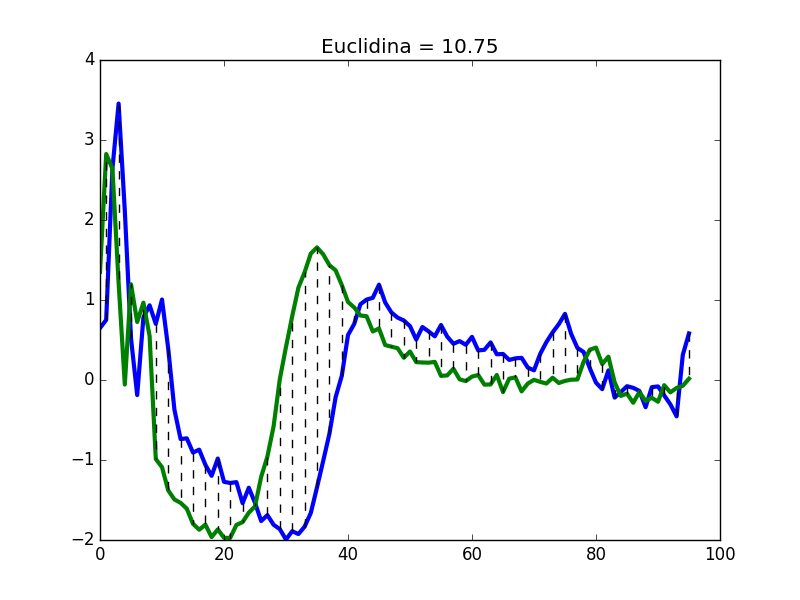
\includegraphics[width=.95\linewidth]{figuras/ECG200_dtw_euclidiana.png}
		\caption{Distância Euclidiana entre duas curvas do conjunto de dados ECG200.}
		\label{fig:sfig1}
%	\end{subfigure}%
\end{figure}
\begin{figure}
%	\begin{subfigure}{.32\textwidth}
		\centering
		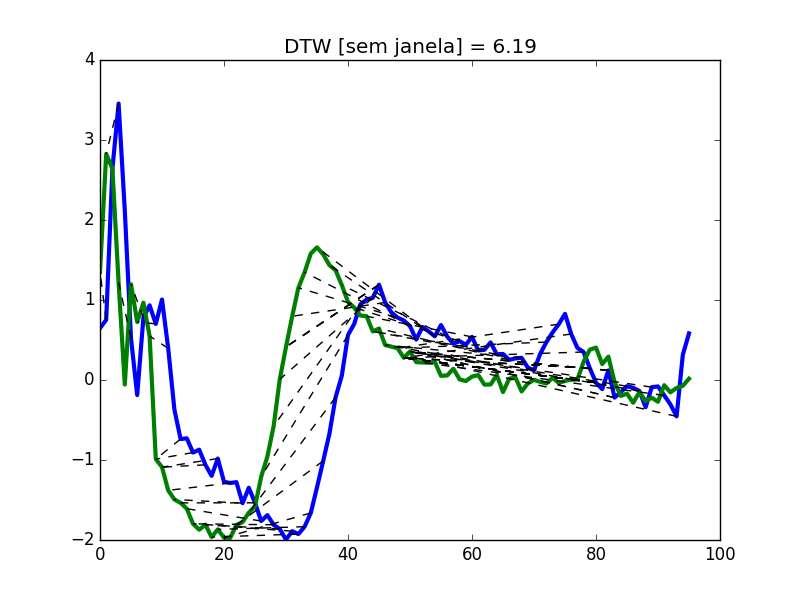
\includegraphics[width=.95\linewidth]{figuras/ECG200_dtw_nowindow.png}
		\caption{DTW sem janela entre duas curvas do conjunto de dados ECG200, na qual foi usada como distância $\delta(x_i,y_j) = (x_i-y_j)^2$..}
		\label{fig:sfig2}
%	\end{subfigure}
\end{figure}
\begin{figure}
	%	\begin{subfigure}{.32\textwidth}
			\centering
			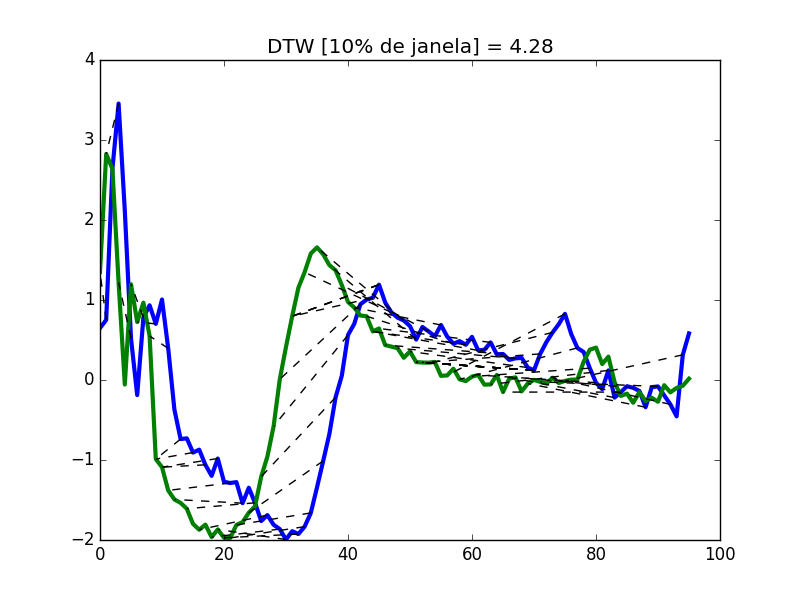
\includegraphics[width=.95\linewidth]{figuras/ECG200_dtw_10_window.png}
			\caption{DTW com janela de tamanho $10\%$ do tamanho da série temporal, entre duas curvas do conjunto de dados ECG200, na qual foi usada como distância $\delta(x_i,y_j) = (x_i-y_j)^2$.}
			\label{fig:sfig3}
		%	\end{subfigure}
%	\caption{Comparação entre as diferentes estratégias para a obtenção da distância euclidiana e dissimilaridade DTW entre duas curvas do conjunto de dados ECG200, na qual foi usada como distância $\delta(x_i,y_j) = (x_i-y_j)^2$. }
	\label{fig:dtw_compare}
\end{figure}

A DTW não pode ser considerada uma métrica de distância pois não obedece à desigualdade do triângulo, no entanto, diferentemente da distância Minkowski, pode ser aplicada à series temporais de diferentes tamanhos e não é sensível ao deslocamentos entre as séries temporais.

Na literatura, a distância Euclidiana é uma das abordagens mais utilizadas para o agrupamento em geral, no entanto, em alguns casos nos quais os dados são séries temporais, ela pode apresentar resultados incoerentes ao se definir a similaridade entre duas séries temporais. Para discutir tal afirmação, os experimentos realizados em ~\parencite{FalhaEuclideana} serão reproduzidos aqui. 

\begin{table}[!h]
	\centering
	\caption{Distâncias euclidiana e DTW entre as curvas da figura ~\ref{fig:euclidiana_falha}.}
	\label{euclidiana_vs_DTW}
	\begin{tabular}{|c|c|c|}
%		\toprule
			\hline
										 				& Euclidiana& DTW\\ 
%		\midrule										 				
			\hline
		(ts1,ts2) 	& 26.95 	& 1.51 \\
					\hline					
		(ts1,ts3) 			& 23.18 	& 1.85 \\
					\hline
		%bottomrule
	\end{tabular}
\end{table}

\begin{figure}[h!]
	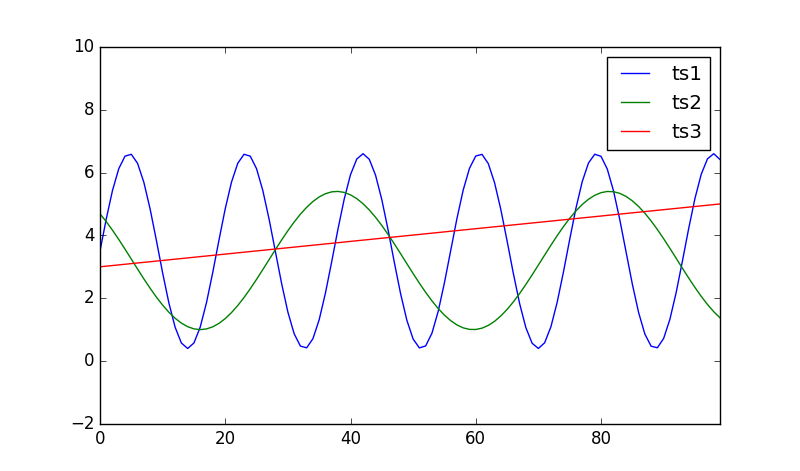
\includegraphics[width=\linewidth]{figuras/euclidiana_falha.png}
	\caption{Duas senóides e uma reta têm suas distâncias comparadas.}
	\label{fig:euclidiana_falha}
\end{figure}
 Na figura ~\ref{fig:euclidiana_falha}, encontram-se três séries temporais e, fixando-se a curva ts1, para compará-la com as outras duas, foram calculadas as distâncias euclidianas e DTW. Os resultados podem ser vistos na tabela ~\ref{euclidiana_vs_DTW}. Pelos dados da tabela, fica claro que a métrica euclidiana falha ao comparar as curvas em análise, já que a distância euclidiana entre a senóide ts1 e a reta ts3 foi menor que a distância euclidiana entre a senoide ts1 e a outra senoide ts2, o que contradiz o nosso senso de similaridade, que é baseado no formato da curva. Por sua vez, a métrica DTW nos diz que a senoide ts1 é mais "próxima"  à senoide ts2 do que à reta ts3, o que condiz com nosso senso de similaridade. A vantagem da DTW em relação à Euclidiana, neste caso, está no fato de a DTW ser invariante à distorção de fase que as curvas podem apresentar entre si.

\subsection{\emph{LB-Keogh}}

A DTW é reconhecida como uma das métricas mais robustas na obtenção da similaridade entre séries temporais, no entanto, seu elevado custo computacional faz com que esta seja preterida em muitas aplicações. Em uma tentativa de se aproximar a DTW com um custo computacional $\mathcal{O}(n)$, em ~\parencite{LB_Keogh} foi proposta a métrica LB-Keogh. No trabalho citado, tal métrica teve resultados próximos à DTW para diversas bases de dados e em tempo significativamente menor. Assim, dada duas séries temporais $\bm{x}$ e $\bm{y}$ de comprimento $n$, então, define-se as séries $\bm{u}$ e $\bm{l}$ como:

\begin{equation} \label{eq:lb_keogh_ini}
\begin{cases}
u_i = \max(y_{i-r}:y_{i+r}),\\
l_i = \min(y_{i-r}:y_{i+r}),
\end{cases}
\end{equation}
onde $r$ é definido como o alcance da aproximação e $1 \leq r \leq n$. As novas séries $\bm{u}$ e $\bm{l}$ formam um envelope que contém a série $\bm{y}$ sendo o limite superior desta formada pela curva $\bm{u}$ e o inferior pela curva $\bm{l}$. Dessa maneira, faz-se necessário que $\forall i \textbf{   } u_i \geq y_i \geq l_i$. Após a definição das duas curvas que formam o envelope, pode-se definir, finalmente, a distância \emph{LB-Keogh} entre as curvas $\bm{x}$ e $\bm{y}$:

\begin{equation} \label{eq:lb_keogh_final}
dist_{LB-Keogh}(\bm{x},\bm{y}) = \sqrt{\sum_{i}^{n} 
	\begin{cases}
	(x_i-u_i)^2,\text{ se }x_i > u_i,\\
	(x_i-l_i)^2,\text{ se }x_i < l_i,,\\
	0, \text{          caso contrário}.\\
	\end{cases}
	}
\end{equation}

A métrica LB-Keogh é sempre menor ou igual ao valor obtido pela DTW, e ao contrário desta última, pode ser aplicada somente em séries temporais de mesmo comprimento e também não pode ser considerada uma métrica de distância pois não obedece à desigualdade do triângulo. Um exemplo de cálculo da LB-Keogh pode ser visto nas figuras ~\ref{fig:keogh_1},~\ref{fig:keogh_2} e ~\ref{fig:keogh_3}.
\begin{figure} 
	\centering
	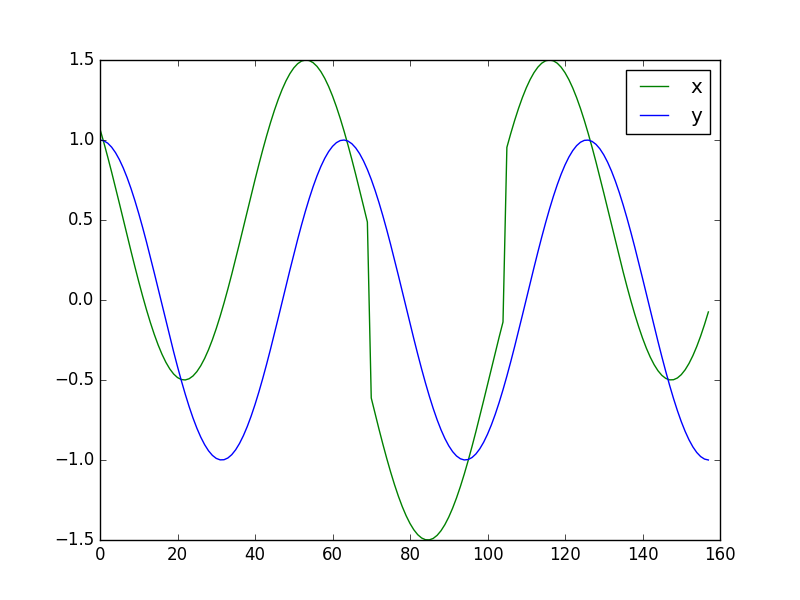
\includegraphics[height=9cm,keepaspectratio]{figuras/lb_keogh_1.png}
	\caption{Curvas $\bm{x}$ e $\bm{y}$.}
	\label{fig:keogh_1}
\end{figure}
\begin{figure}
	\centering
	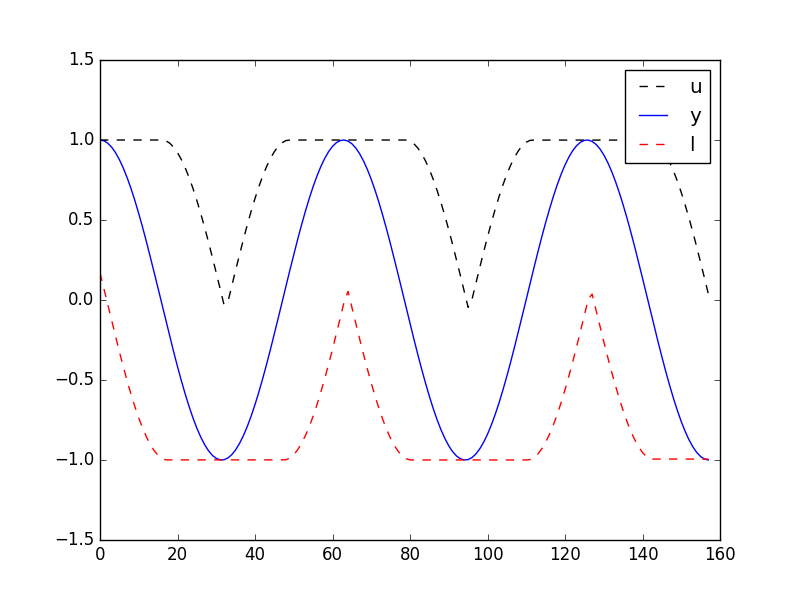
\includegraphics[height=9cm,keepaspectratio]{figuras/lb_keogh_2.png}
	\caption{Curva $\bm{y}$ envelopada pelas curvas $\bm{u}$ e $\bm{l}$ obtidas pela equação ~\ref{eq:lb_keogh_ini}.}
	\label{fig:keogh_2}
\end{figure}
\begin{figure}
	\centering
	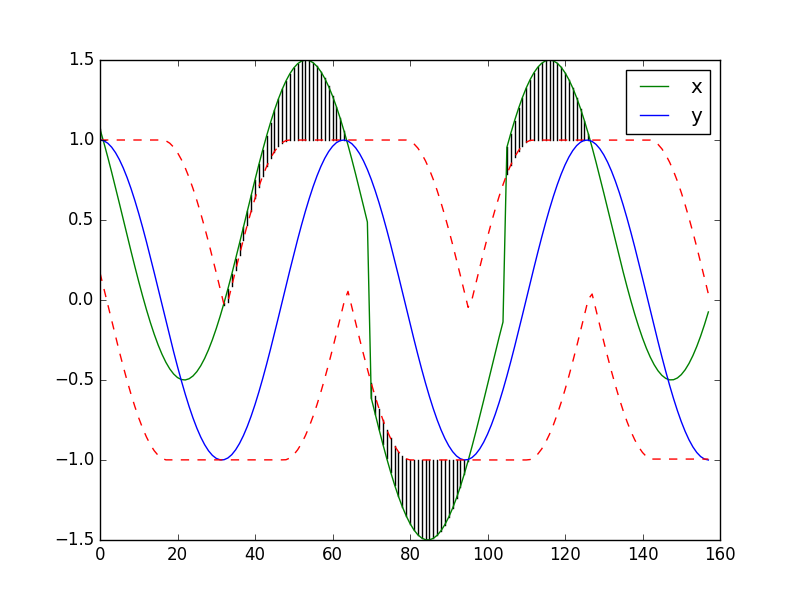
\includegraphics[height=9cm,keepaspectratio]{figuras/lb_keogh_3.png}
	\caption{A raiz do somatório das distâncias em preto fornece a distância LB-Keogh, como descrito pela equação ~\ref{eq:lb_keogh_final}.}
	\label{fig:keogh_3}
\end{figure}

\subsection{\emph{Edit distance on real sequence} - EDR}

Em ~\parencite{EDR}, é proposta uma nova técnica a ser aplicada para a obtenção de métricas de similaridade entre séries temporais multivariadas, com aplicação na análise de trajetórias de objetos móveis. Neste artigo, é defendido que a \emph{Edit distance on real sequence} é uma métrica mais robusta e menos sensível à ruídos e \emph{outliers} que outras métricas tradicionais, como a DTW e a distância Euclidiana.

A métrica é baseada na \emph{Edit distance}, ou distância de \emph{Levenshtein}, que possui larga aplicação na obtenção de métricas de dissimilaridades entre \emph{strings}. A EDR é uma adaptação desta distância a ser aplicada à uma sequência de números reais, ao invés de ser aplicada à uma sequência de caracteres. Apesar de ter sido proposta inicialmente para séries temporais multivariadas, em ~\parencite{Serra} são feitos experimentos com séries temporais univariadas nos quais se chegou a resultados superiores aos resultados de métricas tradicionais como a DTW e distância Euclidiana. Assim como a DTW, a métrica EDR não é sensível ao deslocamento entre as curvas e pode ser utilizada para curvas de comprimentos diferentes.

A EDR de duas curvas de tamanho $m$ e $n$ pode ser obtida por meio da seguinte programação dinâmica:

\begin{equation}
D_{ij} = 
\begin{cases} 
D_{i-1,j-1} 											   & \text{se } c(x_i,y_j) = 1, \\
1 + min(D_{i,j-1},D_{i-1,j},D_{i-1,j-1})     & \text{se } c(x_i,y_j) = 0, \\
\end{cases}
\end{equation}
onde $i=1,...,m$ e $j=1,....n$. A função de casamento $c(x_i,y_j) = \theta (\varepsilon - f(x_i,x_j))$, sendo $\theta(.)$ a função degrau unitário, $\varepsilon \in [0,\infty)$ é um parâmetro a ser escolhido, e sugerido por ~\parencite{EDR} como um quarto da variância da série que possui a maior variância das suas observações, e a função $f(.)$ é normalmente definida como o valor absoluto da diferença entre as variáveis, ou seja, $f(x_i,y_j) = |x_i-y_j|$. Além disso, a matriz $D$ deve ser iniciada da seguinte maneira: $D_{i,0} = i$ para $i=0,1,...,m$ e $D_{0,j} =j$ para $j=0,1,...,n$, e a distância EDR entre as curvas é dado pelo valor contido em $D_{m,n}$.

A EDR não pode ser considerada uma métrica de distância pois não possui a propriedade de desigualdade do triângulo e tem complexidade computacional $\mathcal{O}(m*n)$. Dado o seu elevado custo computacional, restrições devem ser feitas ao cálculo da dissimilaridade.

\subsection{\emph{Dice}, \emph{Jaccard} e \emph{Lorentzian}}

As distâncias \emph{Dice}, \emph{Jaccard} e \emph{Lorentzian} obtiveram performance superior à distância euclidiana em um estudo empírico de classificação de séries temporais realizado em ~\parencite{BatistaComparativo}, e por isso são utilizadas neste trabalho e definidas a seguir. Para duas séries temporais $\bm{x}$ e $\bm{y}$ de comprimento $n$, temos:

\begin{itemize}
	\item Dice \begin{equation}
	dist(\bm{x}, \bm{y}) =\frac{\sum_{i}^{n}(x_i-y_i)^2}{\sum_{i}^{n}x_i^2 + \sum_{i}^{n} y_i^2}
	\end{equation}
		\item Jaccard \begin{equation}
		dist(\bm{x}, \bm{y}) =\frac{\sum_{i}^{n}(x_i-y_i)^2}{\sum_{i}^{n}(x_i^2 +y_i^2-x_i y_i)}
		\end{equation}
			\item Lorentzian \begin{equation}
			dist(\bm{x}, \bm{y}) = \sum_{i}^{n} ln(1 + |x_i-y_i|)
			\end{equation}
\end{itemize}

Todas as três distâncias possuem ordem de complexidade $\mathcal{O}(n)$, e são aplicáveis somente à séries temporais com o mesmo comprimento $n$.

\subsection{\emph{Cosine}}

A métrica \emph{Cosine} é definida  a partir do cosseno do ângulo entre os vetores $\bm{x}$ e $\bm{y}$ das séries temporais:
\begin{equation}
dist(\bm{x},\bm{y}) = 1- \frac{\bm{x}.\bm{y}}{||\bm{x}||_2 ||\bm{y}||_2},
\end{equation}
onde $||\bm{x}||_2$ é a norma euclidiana do vetor $\bm{x}$. A distância \emph{Cosine} tem ordem de complexidade $\mathcal{O}(n)$ e só pode ser calculada em entre séries temporais de mesmo tamanho $n$.

\subsection{Distância de Mahalanobis}

A distância de Mahalanobis é uma distância estatística proposta em ~\parencite{mahalanobis1936generalized}, que leva em conta a covariância entre as amostras da base de dados. Útil na detecção de \emph{outliers}, a distância de Mahalanobis utiliza a matriz de covariância $\Sigma$ das amostras, e, para o caso específico no qual $\Sigma=I$, então a métrica é análoga à distância euclidiana. Assim, a distância de Mahalanobis entre os vetores $\bm{x}$ e $\bm{y}$, pertencentes ao conjunto de dados que gerou a matriz $\Sigma$, é:

\begin{equation}
dist(\bm{x},\bm{y}) = \sqrt{(\bm{x}-\bm{y})^T\Sigma^{-1}(\bm{x}-\bm{y})}.
\end{equation}

Os maiores custos computacionais da obtenção da distância de Mahalanobis residem no cálculo da matriz de covariância $\Sigma$ e da inversão da mesma. Além do custo computacional em si, numericamente, a inversão da matriz $\Sigma$ é problemática pois pode levar a diversos erros numéricos já que, em geral, a matriz $\Sigma$ é de baixo \emph{rank} para conjuntos de dados de séries temporais. O cálculo e inversão da matriz $\Sigma$ têm ordem de complexidade $\mathcal{O}(n^2)$, e a métrica só pode ser aplicada à séries temporais de mesmo tamanho.

Em ~\parencite{mahalanobisClassification}, foi realizado um estudo de classificação de séries temporais no qual a distância de Mahalanobis foi utilizada como métrica de dissimilaridade entre as curvas. Foram realizadas aproximações da inversa da matriz de covariância dos dados que fizeram com que se tivessem ganhos computacionais relevantes, possuindo, assim, custos computacionais inferiores aos custos da DTW, no entanto, com uma pequena perda de performance na acurácia.

\subsection{Distâncias baseadas na correlação de Pearson}

A correlação de Pearson entre duas séries temporais $\bm{x}$ e $\bm{y}$ de tamanho $n$ é dada por

\begin{equation} \label{d_COR}
COR (\bm{x},\bm{y}) = \frac{\sum_{i}^{n}(x_i-\bm{\bar{x}}) (y_i-\bm{\bar{y}})}{\sqrt{\sum_{i}^{n}(x_i-\bm{\bar{x}})^2}\sqrt{\sum_{i}^{n}(y_i-\bm{\bar{y}})^2}},
\end{equation}
sendo $\bar{\bm{x}}$ e $\bar{\bm{y}}$ as média das observações de $\bm{x}$ e $\bm{y}$ respectivamente. O valor da correlação de Pearson é compreendido no intervalo [$-1,1$]. Dessa maneira, as seguintes distância baseadas na correlação de Pearson podem ser definidas

\begin{equation}
dist_1(\bm{x},\bm{y})  = 1-COR(\bm{x},\bm{y}),
\end{equation}

\begin{equation}
dist_2(\bm{x},\bm{y})  = \sqrt{2(1-COR(\bm{x},\bm{y}))},
\end{equation}

\begin{equation}
dist_3(\bm{x},\bm{y}) = \sqrt{\Bigg(\frac{1-COR(\bm{x},\bm{y})}{1+COR(\bm{x},\bm{y})}\Bigg)^\beta},
\end{equation}
onde $\beta$ é um parâmetro para regular o decrescimento da distância $dist_3$. Todas as métricas podem ser aplicadas somente entre séries temporais de mesmo comprimento e possuem ordem de complexidade $\mathcal{O}(n)$, onde $n$ é o número de observações das séries temporais em comparação. 

\subsection{Distância baseada na correlação temporal}

Uma medida da correlação temporal entre duas séries temporais definida em ~\parencite{cort}, é equivalente à uma medida do quão similar é o comportamento dinâmico entre as séries, ou, em outras palavras, o quão próximo está o instante de tempo no qual elas crescem ou decrescem. Definida no intervalo $[-1,1]$ a correlação temporal entre as séries $\bm{x}$ e $\bm{y}$ de tamanho $n$ pode ser obtida por

\begin{equation} \label{d_CORT}
CORT (\bm{x},\bm{y}) = \frac{\sum_{i}^{n-1}(x_i-x_{i+1}) (y_i-y_{i+1})}{\sqrt{\sum_{i}^{n-1}(x_i-x_{i+1})^2}\sqrt{\sum_{i}^{n-1}(y_i-y_{i+1})^2}},
\end{equation}

Valores de correlação temporal próximos de $1$ indicam que as séries $\bm{x}$ e $\bm{y}$ crescem e decrescem simultaneamente e com a mesma taxa, enquanto valores próximos de $-1$ indicam que uma série cresce ao passo que a outra decresce simultaneamente, e isso ocorre com a mesma taxa. Valores próximos de $0$ indicam que estatisticamente não se pode afirmar nada a respeito da taxa e do crescimento ou decrescimento de uma curva ao saber o comportamento da outra.

A partir da equação ~\ref{d_CORT} criar uma métrica que leva em conta tanto aspectos temporais como a correlação temporal quanto a proximidade ponto a ponto entre as séries. Para tal, faz-se uso de uma função de sintonia e de alguma métrica convencional, como a métrica Euclidiana ou DTW, por exemplo. Assim, uma possível métrica de distância que leve em conta o aspecto temporal  entre as séries $\bm{x}$ e $\bm{y}$ seria:

\begin{equation}
dist(\bm{x},\bm{y}) = f(CORT (\bm{x},\bm{y})).dist_Q(\bm{x},\bm{y}) 
\end{equation}
onde $dist_Q$ é a distância convencional entre as séries e $f(.)$ é a função de sintonia que deve amplificar a distância convencional quando a correlação temporal se encontra no intervalo $[-1,0[$, reduzi-la quando a correlação temporal se encontra no intervalo $]0,1]$, e não alterá-la quando a correlação temporal for igual à $0$. A seguinte função, proposta em  ~\parencite{cort}, atende à estes critérios:

\begin{equation} \label{eq:tunning_func}
f(x) = \frac{2}{1+\exp(\gamma x)},\text{ 				} \gamma \geq 0,
\end{equation}
onde $\gamma$ é um parâmetro de controle que controla o quanto o aspecto temporal deve influenciar na métrica de distância. Valores grandes de $\gamma$ fazem com que o valor fornecido por $dist_Q$ seja mais penalizado, ou atenuado, quando se obtém valores não nulos de correlação temporal entre as séries. Tal comportamento da função de sintonia bem como a influência do parâmetro $\gamma$ podem ser vistos na figura ~\ref{fig:tunning_cort}.

Em ~\parencite{cort} são feitos experimentos com séries temporais reais e sintéticas, utilizando-se métricas baseadas na correlação de Pearson e na correlação temporal, e como distâncias convencionais foram escolhidas a DTW e a distância Euclidiana. Após a realização do agrupamento das curvas por meio de algoritmos hierárquicos, utilizando-se as métricas citadas anteriormente, chegou-se à resultados superiores com a correlação temporal utilizando a similaridade DTW como distância convencional. Este resultado superior foi alcançado tanto para os conjuntos de dados sintéticos quanto para o conjunto de dados reais.

A correlação temporal não pode ser considerada uma métrica de distância pois não obedece à desigualdade do triângulo e como o cálculo da correlação temporal tem custo $\mathcal{O}(n)$, seu custo computacional se torna, em geral, o mesmo da distância convencional utilizada. 

\begin{figure}[h!]
	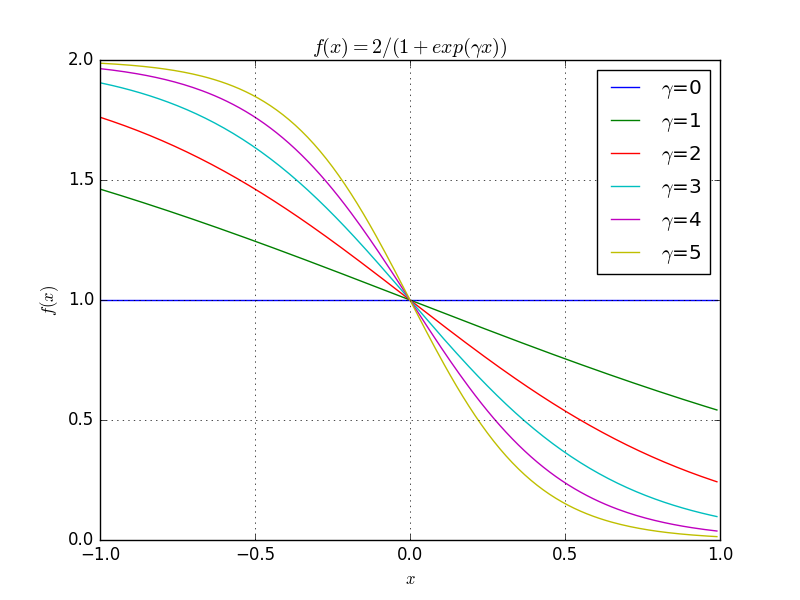
\includegraphics[width=\linewidth]{figuras/tunning_cort.png}
	\caption{Função de sintonia ~\ref{eq:tunning_func} para diferentes valores de $\gamma$.}
	\label{fig:tunning_cort}
\end{figure}

\subsection{\emph{Complex Invariant Distance} - CID} \label{sec:CID}

Em alguns casos, séries temporais "complexas", dependendo da métrica a ser utilizada, podem se tornar mais similares à uma outra série temporal "simples"{} do que à outra série tão "complexa"{} quanto ela. Por complexidade, entende-se uma série temporal com muitos picos e vales ~\parencite{CID}. A \emph{Complex Invariant Distance}, ou CID, leva em conta estimativas de complexidade das séries temporais para realizar uma correção na medida da dissimilaridade e, dessa maneira, para duas séries $\bm{x}$ e $\bm{y}$

\begin{equation}
dist_{CID} = dist_{Q}(\bm{x},\bm{y}) \text{ . } CF(\bm{x},\bm{y}),
\end{equation}
onde $dist_{Q}(.)$ é qualquer uma das dissimilaridades já vistas, como a DTW ou Euclidiana, e $CF(.)$ é um fator de correção que leva em conta uma estimativa da complexidade relativa entre as séries. Note que, pelo fato do fator de correção ser relativo, duas séries que tiverem complexidades semelhantes tenderão a ter um valor muito próximo de $dist_{Q}$, ao passo que séries que possuem complexidades distintas, penalizarão a dissimilaridade $dist_{Q}$.

Em ~\parencite{CID}, é proposto o fator de correção
\begin{equation} \label{eq:CF}
CF (\bm{x},\bm{y}) = \frac{max(CE(\bm{x}),CE(\bm{y}))}{min(CE(\bm{x}),CE(\bm{y}))},
\end{equation}
onde $CE(.)$ é um estimador de complexidade da série temporal.  A complexidade das séries pode ser estimada de diferentes maneiras, como: pela complexidade de Kolmogorov, métricas de entropia, número de trocas do sinal da derivada, entre outras citadas em ~\parencite{TSCLUST}. A medida de complexidade a ser utilizada neste trabalho, sugerida em ~\parencite{CID}, é bastante simples e intuitiva e será obtida pelo comprimento do tamanho da série temporal após esta ser "esticada", e é obtida por 

\begin{equation} \label{eq:CE}
CE(\bm{x}) = \sqrt{\sum_{i}^{n-1} (x_i - x_{i+1})^2}.
\end{equation}

O cálculo do fator de correção possui complexidade $\mathcal{O}(n)$, o que faz com que o custo computacional da métrica seja, em geral, igual ao custo da dissimilaridade $dist_{Q}$, e a pergunta se a dissimilaridade CID pode ou não ser aplicada à séries temporais com diferentes comprimentos, deve ser respondida pela pergunta se a métrica $dist_{Q}$ o faz.

A seguir é exibido um exemplo no qual se faz necessário levar em conta a complexidade entre as séries temporais. Na figura ~\ref{fig:cid} podem ser vistas três séries temporais, sendo uma simples, $ts1$, e duas complexas, $ts2$ e $ts3$. Foram calculadas as distâncias euclidianas e as distâncias euclidianas corrigidas pelo fator de complexidade da Equação ~\ref{eq:CF}. Além dos valores das distâncias euclidianas e CID-euclidiana, na Tabela ~\ref{cid_table}, na primeira coluna, podem ser vistas as complexidades de cada curva. 

Note que, como esperado, as curvas com maior ruído, ou com maior número de picos e vales, possuem complexidade aproximadamente quatro vezes maior do que a curva mais suave, ou mais simples. A submatriz de distância euclidiana entre as curvas nos mostra que as curvas complexas, $ts2$ e $ts3$, estão mais distantes entre si do que da curva mais simples, $ts1$. Tal resultado contradiz nossa intuição de proximidade entre as três curvas analisadas. No entanto, após o fator de correção que leva em conta a complexidade, a distância euclidiana foi corrigida, já que a distância CID-euclidiana entre as curvas complexas é menor que entre cada uma e a curva mais simples, $ts1$.

Este resultado é, em geral, o mesmo para outras métricas de dissimilaridade como a DTW. Em ~\parencite{CID} foi realizado o agrupamento hierárquico de formas geométricas, após estas serem convertidas para séries temporais (vide Figuras ~\ref{fig:cid_1} e ~\ref{fig:cid_2}), e a métrica CID obteve resultados melhores que os resultados com a distância Euclidiana pura, tanto para dados sintéticos como para dados reais. No teste de classificação empírico realizado em ~\parencite{BatistaComparativo}, a CID, utilizando a DTW como distância convencional, obteve a melhor acurácia dentre outras 45 métricas utilizada, para 20 conjuntos de dados de séries temporais diferentes.

\begin{figure}[h!]
	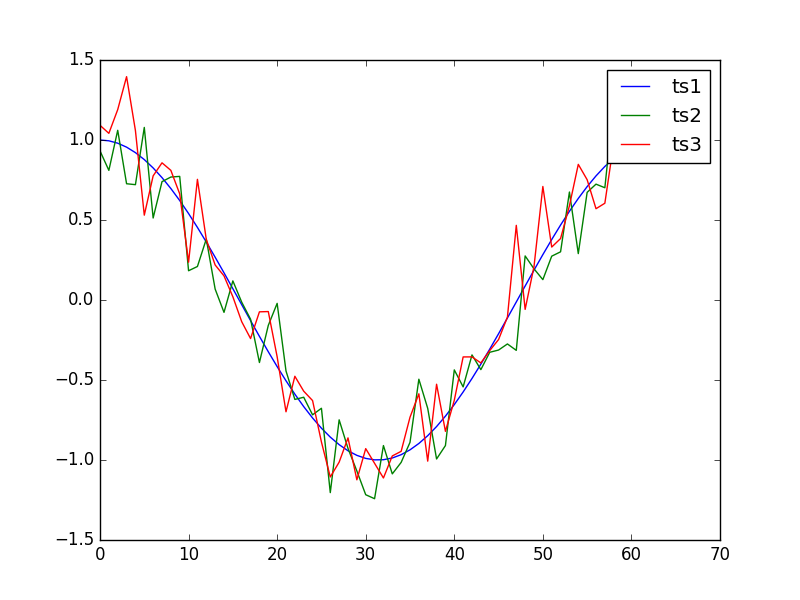
\includegraphics[width=\linewidth]{figuras/CID.png}
	\caption{Três curvas diferentes sendo duas complexas e uma simples. A estimativa de complexidade de cada uma bem como as distâncias CID e euclidiana entre elas podem ser vistas na tabela ~\ref{cid_table}}
	\label{fig:cid}
\end{figure}

\begin{table}[!h]
	\centering
	\caption{Medida de complexidade, como definida na equação ~\ref{eq:CE}, das curvas da figura ~\ref{fig:cid} e distâncias euclidiana e CID-euclidiana entre elas.}
	\label{cid_table}
	\begin{tabular}{c|c|ccc|ccc}
		%\begin{tabular}{llllllll}
		\toprule
		& Complex.  & Eucl.(ts1)   & Eucl.(ts2)   &Eucl.(ts3)  & CID.(ts1)   & CID.(ts2)   &CID.(ts3) \\
		\midrule

ts1 & 0.560 & 0.0 & 1.408 & 1.354 & 0.0 & 5.090 & 4.777\\
ts2 & 2.025 & 1.408 & 0.0 & 2.027 & 5.090 & 0.0  & 2.078\\		
ts3 & 1.975 & 1.354 & 2.027 & 0.0 & 4.777 & 2.078  & 0.0\\
		\bottomrule
	\end{tabular}
\end{table}

\subsection{Discussão geral das métricas de dissimilaridade}

Após a exposição das diversas métricas de dissimilaridade, faz-se necessária a sumarização de todas as informações nesta seção, que pode ser vista na Tabela ~\ref{tbl:dissimlarity_summary_table}, bem como de uma discussão geral acerca das métricas de dissimilaridade entre séries temporais. A escolha da métrica a ser utilizada no agrupamento depende sensivelmente do domínio do problema e de como a série temporal foi gerada. Para algumas aplicações, em que o formato da série é relevante, métricas que medem a dissimilaridade ponto a ponto são mais indicadas. Em contrapartida, para aplicações onde o interesse é verificar se as séries crescem ou decrescem de forma similar, independentemente do seu formato, métricas baseadas em correlação temporal são mais apropriadas. Além disso, as séries temporais a serem agrupadas, ou classificadas, podem possuir diversas distorções, devido à sua natureza ou pela maneira que elas foram obtidas, e isso deve ser levado em conta na escolha da métrica, uma vez que determinadas métricas são naturalmente invariantes a algumas distorções.

Em problemas de mineração de dados de séries temporais, é desejável que a métrica de dissimilaridade e o pré-processamento escolhidos alcancem uma ou mais das seguintes invariâncias, que são detalhadas em \parencite{CID} e serão brevemente discutidas nas subseções seguintes. Vale ressaltar que ao se tentar remover algumas das distorções em um problema específico, resultados piores podem ser obtidos, de forma que cada conjunto de dados de séries temporais deve ser analisado antes de se definir quais invariâncias são necessárias para a comparação entre as séries temporais.

\subsubsection{Invariância à amplitude/\emph{offset}}

Quando as séries temporais a serem comparadas são idênticas, mas medidas com diferentes escalas, estas possuem amplitudes distintas, e as métricas de dissimilaridades já discutidas podem apresentar valores muito altos, o que pode indicar erroneamente que as séries são dissimilares. Além da amplitude, séries que são idênticas, mas possuem um valor médio diferente (\emph{offset}), podem apresentar também valores muito grandes de dissimilaridade. A solução apresentada em \parencite{CID}, e discutida na seção ~\ref{sec:norm_Z}, para se alcançar a invariância à amplitude e \emph{offset} é a utilização da normalização Z nas curvas das séries temporais, em uma etapa de pré-processamento. Exemplos de curvas que devem ser comparadas com invariância à amplitude e \emph{offset} podem ser vistas na Figura ~\ref{fig:inv_offset_amplitude}.

\begin{figure}[h!]
	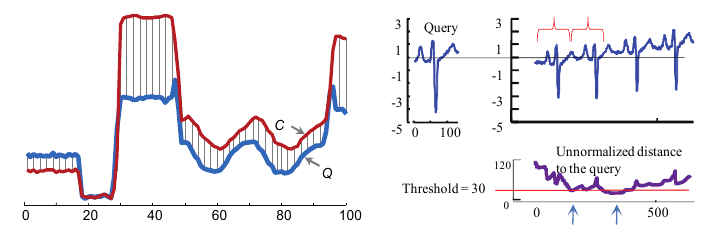
\includegraphics[width=\linewidth]{figuras/invariancias/amplitude_offset.png}
	\caption{À esquerda duas curvas, não normalizadas, que, quando comparadas, se parecem bastante distintas, quando na verdade não o são. À direita um eletrocardiograma, a ser comparado com um sinal de medição contínuo. As duas primeiras comparações têm um bom casamento, mas as subsequentes apresentam valores maiores em uma comparação ponto a ponto devido ao crescente \emph{offset} que a curva começa a apresentar. Extraído de ~\parencite{CID}}
	\label{fig:inv_offset_amplitude}
\end{figure}

\subsubsection{Invariância à escala local ou ao deslocamento}

Muito comum em sinais biológicos, a invariância à escala local ou ao deslocamento das séries, se manifesta quando o alinhamento ótimo entre as séries ocorre devido à um entortamento local. A dissimilaridade DTW é uma métrica invariante ao deslocamento, e tal propriedade pode ser vista na Figura ~\ref{fig:dtw_compare}

\begin{figure}[h!]
	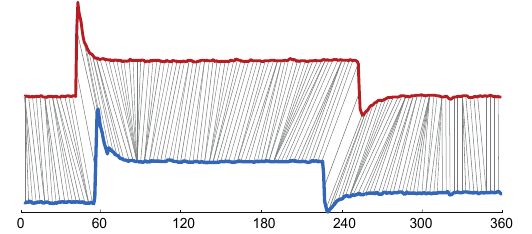
\includegraphics[width=\linewidth]{figuras/invariancias/deslocamento.png}
	\caption{Duas curvas cujo alinhamento ótimo é obtido por meio da DTW. Extraído de ~\parencite{CID}}
	\label{fig:inv_deslocamento}
\end{figure}


\subsubsection{Invariância à escala uniforme}

Em alguns casos, duas séries temporais que são idênticas ou da mesma classe mas, por questões de medição, possuem tamanhos distintos, podem ter sua dissimilaridade afetada ao se utilizar alguma métrica de dissimilaridade como a DTW, por exemplo. A solução apresentada em \parencite{CID} para tal é a multiplicação de uma das curvas por um fator $\kappa$, que irá esticar ou reduzir uma das curvas para melhorar o casamento entre elas. A principal dificuldade em se obter a invariância à escala uniforme na comparação de séries temporais é a definição do valor de $\kappa$, que na prática, é obtido por meio de diversos testes dentro de determinado intervalo na etapa de pré-processamento. Um alinha mento ótimo obtido por meio da escala uniforme pode ser visto na Figura ~\ref{fig:inv_escala_uniforme}.

\begin{figure}[h!]
	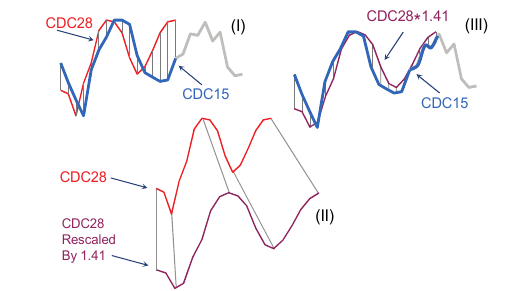
\includegraphics[width=\linewidth]{figuras/invariancias/escala_uniforme.png}
	\caption{Duas curvas cujo alinhamento ótimo é obtido após a curva ser esticada por um fator $\kappa=1.41$, que foi obtido por força bruta. Extraído de ~\parencite{CID}.}
	\label{fig:inv_escala_uniforme}
\end{figure}

\subsubsection{Invariância ao defasamento}

A invariância ao defasamento é muito importante quando se compara duas séries temporais periódicas. Segundo \parencite{CID} algumas heurísticas foram propostas para se obter a invariância ao defasamento entre duas séries temporais, mas nenhuma delas é robusta o suficiente, de forma que tal invariância deve ser obtida por meio do teste de todos os alinhamentos possíveis entre as curvas na etapa de pré-processamento. Dessa maneira, este é um problema em aberto na literatura, e nenhuma das dissimilaridades ou técnicas de pré-processamento discutidas alcançam a invariância ao deslocamento. A Figura ~\ref{fig:inv_defasamento} demonstra a obtenção desta invariância para duas séries temporais.

\begin{figure}[h!]
	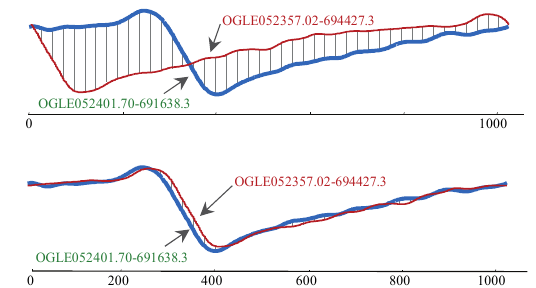
\includegraphics[width=\linewidth]{figuras/invariancias/defasamento.png}
	\caption{Duas curvas que após sucessivas tentativas de defasamento de uma delas, possuem casamento ótimo. Cada uma delas representa dados de radiação colhidos de uma estrela diferente. Extraído de ~\parencite{CID}.}
	\label{fig:inv_defasamento}
\end{figure}

\subsubsection{Invariância à oclusão}

Algumas séries temporais podem apresentar subsequências que não possuem valores observados, por algum erro na medição, ou pela própria característica do problema. A invariância à oclusão pode ser obtida ao se ignorar determinadas partes das séries temporais que não possuem casamento. Algumas métricas de dissimilaridade como a DTW e EDR são mais robustas à oclusão do que a distância Euclidiana. A comparação entre as séries temporais geradas a partir das imagens de dois crânios, na qual se faz necessária a invariância à oclusão, pode ser vistas na Figura ~\ref{fig:inv_oclusao}.

\begin{figure}[h!]
	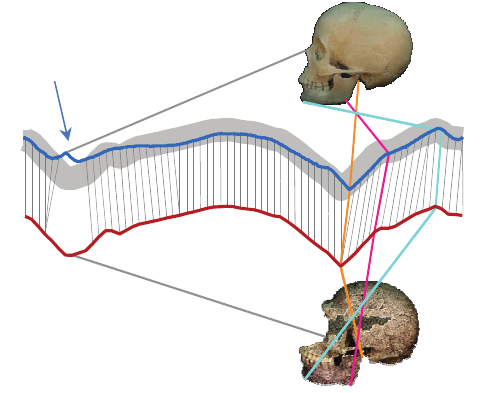
\includegraphics[width=\linewidth]{figuras/invariancias/oclusao.png}
	\caption{Duas curvas geradas a partir do formato de dois crânios a serem comparados. A falta da região do nariz de um dos crânios pode influenciar significativamente na comparação entre as métricas. Extraído de ~\parencite{CID}.}
	\label{fig:inv_oclusao}
\end{figure}

\subsubsection{Invariância à complexidade}

A complexidade de uma série temporal, como definida na seção \ref{sec:CID}, diz respeito ao número de picos e vales que a série apresenta. Observa-se que em diferentes domínios, instâncias de diferentes classes possuem complexidades distintas, o que torna tal atributo da série temporal relevante para as tarefas de classificação e agrupamento destas. A melhor maneira de se levar em conta as complexidades das séries temporais ao compará-las, é a utilização do fator de correção CID exposto na seção ~\ref{sec:CID}. As figuras ~\ref{fig:cid_1} e ~\ref{fig:cid_2} demonstram um problema no qual a invariância à complexidade influencia os resultados em uma tarefa de agrupamento.

\begin{figure}[h!]
	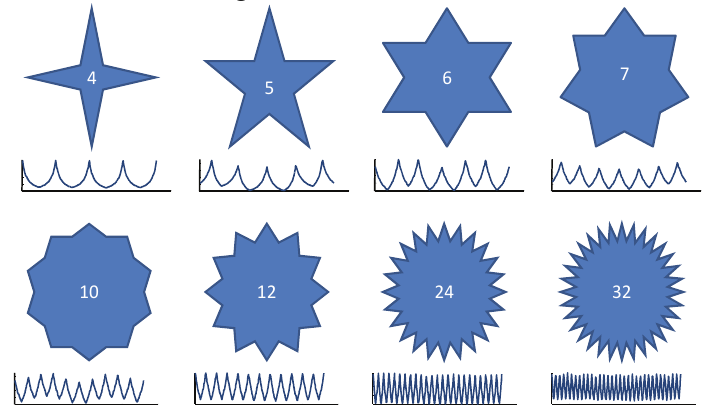
\includegraphics[width=\linewidth]{figuras/invariancias/cid_1.png}
	\caption{Diversas formas geométricas e as séries temporais geradas para cada uma delas. As curvas foram geradas pela distância do ponto central da figura até cada ponto do seu contorno. Extraído de ~\parencite{CID}.}
	\label{fig:cid_1}
\end{figure}
\begin{figure}[h!]
	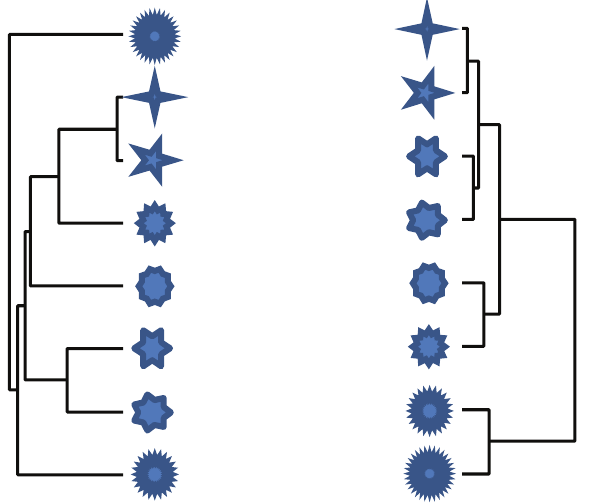
\includegraphics[width=\linewidth]{figuras/invariancias/cid_2.png}
	\caption{Agrupamentos hierárquicos com \emph{linkagem} average realizados nas curvas; à esquerda com a distância euclidiana e à direita com a distância euclidiana corrigida pela CID. Extraído de ~\parencite{CID}.}
	\label{fig:cid_2}
\end{figure}

\begin{table}[!h]
	\centering
	\caption{Sumário das métricas de dissimilaridades discutidas em ~\ref{sec:metricas}.}
	\label{tbl:dissimlarity_summary_table}
	\resizebox{\columnwidth}{!}{%
	\begin{tabular}{ccccccc}
		%\begin{tabular}{llllllll}
		\toprule
		Métrica 		& Distância? 		& Ordem de complexidade & Inv. Oclusão & Inv. Deslocamento & Inv. Complexidade & Ref. \\
		\midrule
		Minkowski 	  & 	\checkmark & $\mathcal{O}(n)$			 & {} 				 & {}						& {} 						 & \parencite{DudaHart} \\
		DTW			    & 	{}      		   & $\mathcal{O}(n_1*n_2)$ 		   & {} 			   &  \checkmark     & {} 						 & \parencite{DTW} \\
		LB-Keogh	& 	{}      		   & $\mathcal{O}(n)$ 		   & {} 			   &  \checkmark     & {} 				& \parencite{LB_Keogh} \\
		EDR			    & 	{}      		   & $\mathcal{O}(n_1*n_2)$ 		   & {} 			   &  \checkmark     & {} 						 & \parencite{EDR} \\
		Dice	& 	{}      		   & $\mathcal{O}(n)$ 		   & {} 			   & {}    & {} 				& \parencite{BatistaComparativo} \\
		Jaccard	& 	{}      		   & $\mathcal{O}(n)$ 		   & {} 			   &  {}     & {} 				& \parencite{BatistaComparativo} \\
		Lorentzian	& 	{}      		   & $\mathcal{O}(n)$ 		   & {} 			   &  {}     & {} 				& \parencite{BatistaComparativo} \\
		Cosine	& 	{}      		   & $\mathcal{O}(n)$ 		   & {} 			   &  {}     & {} 				& \parencite{BatistaComparativo} \\
		Mahalanobis	& 	{}      		   & $\mathcal{O}(n^2)$ 		   & {} 			   &  {}     & {} 				& \parencite{mahalanobis1936generalized} \\
		Pearson	& 	{}      		   & $\mathcal{O}(n)$ 		   & {} 			   &  {}     & {} 				& \parencite{TSCLUST} \\
		CORT			      & 	{}      	& $\mathcal{O}(n)$ 		   & {} 			   &  {}                      & {}				         	 & \parencite{cort} \\
		CID			      & 	{}      		  & $\mathcal{O}(n)$ 		   & {} 			   &  {}                      & \checkmark         	 & \parencite{CID} \\
		\midrule
	\end{tabular}
} % --> resizebox
\end{table}

\section{Algoritmos de agrupamento}

Dada uma métrica de dissimilaridade e um conjunto de dados, existem diferentes algoritmos que realizam a tarefa de agrupamento dos dados, e segundo ~\parencite[][243]{Ullman} estes podem ser divididos em:

\begin{enumerate}
	\item  algoritmos hierárquicos ou aglomerativos, nos quais, inicialmente, cada instância representa um grupo formado por apenas ela mesma, e a partir daí os grupos são combinados sucessivamente a partir de um critério que leva em conta a dissimilaridade entre os grupos,
	\item algoritmos particionais, ou de atribuição de pontos, nos quais cada ponto, ou instância, é atribuído inicialmente à um grupo de uma solução inicial. Em seguida, os pontos são iterativamente realocados entre os grupos, até determinado critério de parada para a obtenção da partição final. Quando os pontos são atribuídos a somente um grupo, dá-se o nome de \emph{hard-clustering}, enquanto quando atribui-se graus de pertinência do ponto à cada um dos grupos, têm-se o \emph{soft-clustering}, ou \emph{fuzzy clustering}.
\end{enumerate}
Os algoritmos de agrupamento podem ser, ainda, classificados em:

\begin{enumerate}
	\item algoritmos que assumem que as instâncias se encontram no espaço euclidiano, ou seja, que a métrica de dissimilaridade utilizada é a distância Euclidiana. Essa distinção existe pois no espaço euclidiano existe o conceito de centróide, que é o ponto médio das instâncias que compõem o grupo, e este ponto é tido como o ponto mais representativo deste. Note que este ponto mais representativo não é, necessariamente, um ponto do conjunto de dados. Assim, em espaços não euclidianos, tal conceito de um ponto médio não existe e, dessa maneira, deve-se utilizar outras estratégias para se definir um ponto representativo dos grupos.
	\item algoritmos que assumem que os dados são pequenos, o suficiente, no que diz respeito ao consumo de memória, para serem armazenados na memória RAM. Caso isso não seja verdade, outras estratégias já partem do pressuposto que é inviável mensurar a dissimilaridade entre todos os pontos, de maneira que diversos algoritmos já são descartados. 
\end{enumerate}

Além dos critérios supracitados, os algoritmos de agrupamento podem, ainda, serem classificados em: aqueles baseados em características, nos quais exigem como entrada uma matriz $NxD$ contento os dados, que são formados por $N$ instâncias, sendo cada uma composta por $D$ características, e os algoritmos de agrupamento baseados em dissimilaridades, os quais esperam uma matriz simétrica $NxN$, onde o elemento $ij$ desta matriz contém a dissimilaridade entre o i-ésimo e o j-ésimo elemento da matriz $NxD$ que contém as instâncias. A seguir seguem breves comentários de alguns dos principais algoritmos de agrupamento utilizados no contexto de agrupamento de séries temporais.

\subsection{Algoritmos particionais}

\subsubsection{\emph{k-means}}

O \emph{k-means}, ou k-médias, ou algoritmo de Lloyd, é uma heurística que utiliza o conceito de centróide para a obtenção da partição final. Basicamente, dado um número $k$ de grupos, o objetivo do algoritmo é encontrar uma partição dos dados que minimize o soma do quadrado da distância entre as instâncias de cada grupo e seu centróide. A resolução deste problema é NP-difícil, no entanto em ~\parencite{Lloyd} é proposto um algoritmo de busca local que fez com que o \emph{k-means} se tornasse um dos algoritmos de agrupamento mais populares.

O algoritmo \emph{k-means} se encontra detalhado no pseudocódigo ~\ref{alg:k_means}, e pelo fato de ser um algoritmo de busca local, deve ser executado diversas vezes, para tentar se chegar ao mínimo global. O \emph{k-means} foi o precursor de diversas outras técnicas de agrupamento, que são variações dele ou outras técnicas realmente inspiradas no \emph{k-means}. Dentre as principais podemos destacar: \emph{k-means++} ~\parencite{k-means++} , \emph{k-medoids} ~\parencite{k-medoids} e \emph{Fuzzy-k-means } ~\parencite{fuzzy_k-means}.

Uma das desvantagens do \emph{k-means} é que se deve definir \emph{a priori} o número de grupos da partição. Essa informação nem sempre se encontra disponível de antemão, o que faz com que sejam realizadas partições com valores iterativos de $k$, e a partir dos valores dos índices de validação de agrupamento, pode-se ter uma ideia do melhor valor de $k$, dentro de determinado intervalo.

A utilização do \emph{k-means} para o agrupamento de séries temporais fica limitada para os casos nos quais a distância euclidiana foi utilizada como métrica de dissimilaridade entre as instâncias, pois somente no espaço euclidiano faz sentido a utilização de pontos médios ou centroides. Em outras palavras, isso significa que várias das métricas promissoras detalhadas na seção ~\ref{sec:metricas}, como a DTW, CID, entre outras, não podem ser utilizadas no agrupamento por meio do algoritmo \emph{k-means}.

\begin{algorithm}
	\caption{Algoritmo \emph{k-means}.}
	\label{alg:k_means}
	\begin{algorithmic}[1]
	\STATE{\textbf{Entradas:  número k de grupos, matriz X de dados com n instâncias e critério de parada $\epsilon$}}
		\STATE{\textbf{Saída:  partição $\mathcal{G}$ dos dados }}
	
	\FOR{$i \leftarrow 1$ \TO $k$}
		\STATE{$j \leftarrow rand(0,n)$} // escolhe aleatoriamente um índice da matriz de dados
		\STATE{$\mathcal{C}_i \leftarrow {x_j}$} //define o centróide como a instância escolhida;
		\STATE{$\mathcal{G}_i \leftarrow {\emptyset}$} // Inicia o i-ésimo grupo vazio
	\ENDFOR
	
	\STATE{$\phi \leftarrow \epsilon $}	// soma das distâncias de cada ponto ao seu centroide

	\WHILE{$\phi \geq \epsilon$}	
		\FOR{$p \leftarrow 1$ \TO $n$}
				\FOR{$i \leftarrow 1$ \TO $k$}
						\STATE{$d_i \leftarrow {dist(x_p,C_i)}$} // calcula a distância do ponto a cada centroide
				\ENDFOR
			
				\STATE{$ s \leftarrow {\arg \min_{i} (d_i)}$}	// Encontra o centroide mais próximo ao ponto p
				\STATE{$\mathcal{G}_s \leftarrow {x_p}$} // Associa o ponto p ao grupo do seu centroide mais próximo			
		\ENDFOR

		\STATE{$\phi \leftarrow 0$}	// soma das distâncias de cada ponto ao seu centroide
		\FOR{$i \leftarrow 1$ \TO $k$}
			\STATE{$\mathcal{C}_i \leftarrow {centroid(\mathcal{G}_i)}$} // Atualiza o centroide do i-ésimo grupo
			\FOR{$j \leftarrow 1$ \TO $n$}			
				\IF{$x_j \in \mathcal{G}_i$}
					\STATE{$\phi \leftarrow \phi + dist(x_j,C_i)$}	// soma das distâncias de cada ponto ao seu centroide
				\ENDIF
			\ENDFOR
		\ENDFOR
		
	\ENDWHILE
		
	\end{algorithmic}
\end{algorithm}

\subsubsection{\emph{K-medoids}}

Essencialmente, o \emph{k-medoids} é uma variação do \emph{k-means}, na qual a única diferença é que não se faz o uso de um ponto médio, ou centróide, das instâncias de um mesmo grupo, mas sim de um ponto mediano, ou medóide, que melhor representa as instâncias de cada grupo. O algoritmo se encontra detalhado no pseudocódigo ~\ref{alg:k_medoids}, onde pode ser visto que a única diferença em relação ao pseudocódigo ~\ref{alg:k_means} se encontra na linha $18$, ao realizar a atualização dos medóides de cada grupo, ao invés da atualização dos centróides.  Dessa maneira, diferentemente do \emph{k-means}, o \emph{k-medoids} consegue trabalhar com qualquer métrica de dissimilaridade, além da distância euclidiana.

O medóide pode ser definido de diversas maneiras, sendo a mais comum como a instância do grupo cuja a soma da distância, ou dissimilaridade, entre ela e as demais instâncias do  mesmo grupo é mínima para aquele grupo ~\parencite[][253]{Ullman}. Então dado um conjunto de dados $X$ composto por $n$ instâncias $x_i, i=0,...,n$, o medóide $x_{med}$ é definido como

\begin{equation}
x_{med} = \arg \min_{x_i} \sum_{j=0}^{n} diss(x_i,x_j), \text{			}i=0,...,n
\end{equation}

\begin{algorithm}
	\caption{Algoritmo \emph{k-medoids}.}
	\label{alg:k_medoids}
	\begin{algorithmic}[1]
		\STATE{\textbf{Entradas:  número k de grupos, matriz X de dados com n instâncias e critério de parada $\epsilon$}}
		\STATE{\textbf{Saída:  partição $\mathcal{G}$ dos dados }}
		
		\FOR{$i \leftarrow 1$ \TO $k$}
		\STATE{$j \leftarrow rand(0,n)$} // escolhe aleatoriamente um índice da matriz de dados
		\STATE{$\mathcal{C}_i \leftarrow {x_j}$} //define o medóide como a instância escolhida;
		\STATE{$\mathcal{G}_i \leftarrow {\emptyset}$} // Inicia o i-ésimo grupo vazio
		\ENDFOR
		
		\STATE{$\phi \leftarrow \epsilon $}	// soma das distâncias de cada ponto ao seu medóide
		
		\WHILE{$\phi \geq \epsilon$}	
		\FOR{$p \leftarrow 1$ \TO $n$}
		\FOR{$i \leftarrow 1$ \TO $k$}
		\STATE{$d_i \leftarrow {dist(x_p,C_i)}$} // calcula a distância do ponto a cada medóide
		\ENDFOR
		
		\STATE{$ s \leftarrow {\arg \min_{i} (d_i)}$}	// Encontra o medóide mais próximo ao ponto p
		\STATE{$\mathcal{G}_s \leftarrow {x_p}$} // Associa o ponto p ao grupo do seu medóide mais próximo			
		\ENDFOR
		
		\STATE{$\phi \leftarrow 0$}	// soma das distâncias de cada ponto ao seu medóide
		\FOR{$i \leftarrow 1$ \TO $k$}
		\STATE {\textbf{$\mathcal{C}_i \leftarrow {medoid(\mathcal{G}_i)}$}} // Atualiza o medóide do i-ésimo grupo
		\FOR{$j \leftarrow 1$ \TO $n$}			
		\IF{$x_j \in \mathcal{G}_i$}
		\STATE{$\phi \leftarrow \phi + dist(x_j,C_i)$}	// soma das distâncias de cada ponto ao seu medóide
		\ENDIF
		\ENDFOR
		\ENDFOR
		
		\ENDWHILE
		
	\end{algorithmic}
\end{algorithm}

\subsection{Algoritmos hierárquicos}

Os algoritmos hierárquicos, possuem a vantagem de não ser necessário informar, \emph{a priori}, o número de grupos que os dados se encontram divididos, no entanto, em geral, possuem ordem de complexidade de  $\mathcal{O}(n^2log(n))$, onde $n$ é o número de instâncias, e esta complexidade é superior em relação aos algoritmos baseados em atribuição de pontos. Outra característica relevante dos algoritmos de agrupamento hierárquicos é que estes são determinísticos, ou seja, para uma mesma entrada, e mesmos parâmetros, sempre retornam a mesma partição. Eles conseguem trabalhar tanto com matrizes de características como com matrizes de dissimilaridade ~\parencite[][245]{Ullman}.

Os algoritmos hierárquicos podem ser divididos em algoritmos divisivos ou aglomerativos. Nos primeiros, inicialmente é considerado um grande grupo que contém todos os dados e que é iterativamente particionado até que cada instância esteja contida em grupo formado única e exclusivamente por ela mesma. Já nos algoritmos aglomerativos ocorre o processo inverso, no qual, inicialmente, cada instância está contida única e exclusivamente em seu próprio grupo, e iterativamente os grupos são fundidos para formar um novo grupo, até que se tenha somente um grande grupo contendo todos os dados. O pseudocódigo de um algoritmo hierárquico aglomerativo se encontra detalhado em ~\ref{alg:aglomerative_clustering}.

O resultado de ambas as abordagens, é a estrutura de uma árvore binária chamada dendrograma, na qual as instâncias se encontram nas folhas da árvore e os ramos representam a união sucessiva das instâncias em um mesmo grupo. O tamanho do ramo que une dois grupos representa a distância, ou dissimilaridade, entre eles, de forma que ramos maiores representam uma maior distância entre os grupos. Dessa maneira, visualmente, pela altura dos ramos em um dendrograma, é possível se ter uma ideia do número de grupos que melhor representa a partição dos dados. Um exemplo de dendrograma pode ser visto na figura ~\ref{fig:dendrograma_exemplo}, o qual é resultado do agrupamento hierárquico com a \emph{linkagem} average, que será melhor detalhada a seguir, e métrica de dissimilaridade euclidiana para o famoso conjunto de dados Iris ~\parencite{Iris}.

\begin{figure}[h!]
	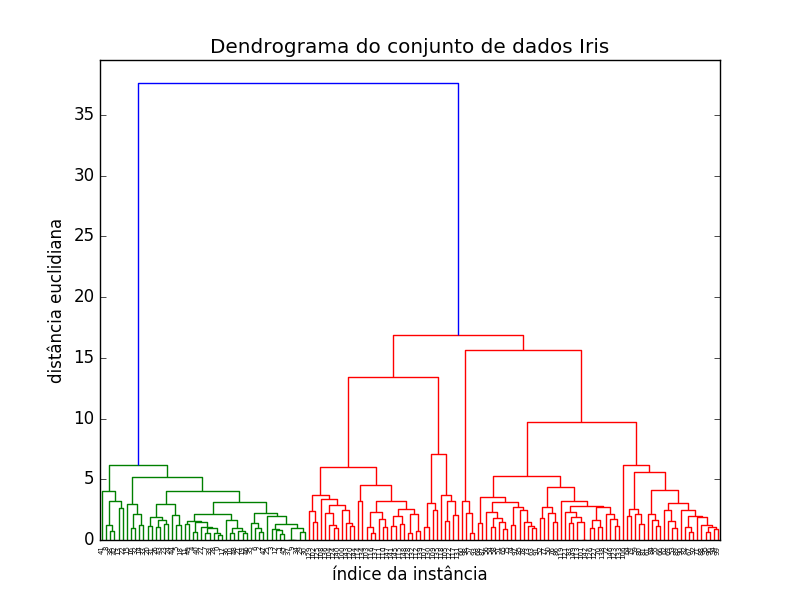
\includegraphics[width=\linewidth]{figuras/dendrograma_exemplo.png}
	\caption{Exemplo de um dendrograma resultante do agrupamento hierárquico com a \emph{linkagem} average e métrica de dissimilaridade euclidiana para o conjunto de dados Iris.}
	\label{fig:dendrograma_exemplo}
\end{figure}

\begin{algorithm}
	\caption{Agrupamento aglomerativo.}
	\label{alg:aglomerative_clustering}
	\begin{algorithmic}[1]
		
		\STATE{\textbf{Entradas:  matriz X de dados com n instâncias}}
		\STATE{\textbf{Saída:  partição $\mathcal{C}$ dos dados }}
	%	\renewcommand{\REQUIRE}{\textbf{Entradas: }}
	%	\REQUIRE \text{Matriz quadrada de similaridade d de dimensão n}
%		\STATE
		\FOR{$i \leftarrow 1$ \TO $n$} 
			\STATE{$\mathcal{C}_i \leftarrow {i}$} //inicializa cada grupo;
		\ENDFOR
		\STATE $\mathcal{S} \leftarrow \{1,..,n\}$; // inicializa o conjunto de grupos a serem aglomerados;
		\WHILE{$|\mathcal{S}| > 1$}
			\STATE{$(j,k) \leftarrow arg \min_{j,k \in \mathcal{S}} d_{j,k} $}; //Escolhe os dois grupos mais similares
			\STATE{$\mathcal{C}_l \leftarrow \mathcal{C}_j \cup \mathcal{C}_k$}; // Cria o novo grupo
			\IF{$\mathcal{C}_l \neq \{1,...,n\}$}
				\STATE{$\mathcal{S} \leftarrow \mathcal{S} \cup \{l\}$}; // Marca o novo grupo como disponível para algomeração
			\ENDIF
			\renewcommand{\algorithmicforall}{\textbf{foreach}}
			\FORALL{$i \in \mathcal{S}$}
				\STATE{d(i,l)} ; // Atualiza a matriz de similaridade
			\ENDFOR			
		\ENDWHILE
		
	\end{algorithmic}
\end{algorithm}

Existem três variações principais na maneira de se definir a dissimilaridade entre os grupos, e cada uma delas pode acarretar em resultados bastante diferentes. A seguir seguem breves comentários de cada uma delas. 

Na abordagem \emph{Single link}, a distância entre dois grupos é definida como a menor distância entre duas instâncias de cada grupo. Por sua vez, na \emph{Complete link}, a distância entre dois grupos é a maior distância entre duas instâncias de cada grupo. Assim, se o diâmetro de um grupo é definida como a maior distância entre instâncias contidas no grupo, então a abordagem \emph{complete link} gera partições com grupos bastante compactos mas pouco dispersos, enquanto a estratégia \emph{single link} cria partições com agrupamentos pouco compactos mas muito dispersos entre si.

 Em uma tentativa de se alcançar as virtudes de ambos os métodos, foi proposta a \emph{average link}, no qual a distância entre dois grupos é definida como a distância média das distâncias entre todos os pares de instâncias que formam o grupo. Na prática, a abordagem \emph{average link} é a mais utilizada por obter partições que representam um compromisso entre compactação e dispersão dos dados.


\subsection{Algoritmos baseados em densidades}

Os algoritmos particionais possuem a grande desvantagem de ser necessário o conhecimento, \emph{a priori}, do número $k$ de grupos que os dados se encontram naturalmente particionados. Dessa maneira, faz-se necessário rodadas iterativas com diferentes valores de $k$ para se alcançar a partição desejada, o que em muitas aplicações, principalmente para aquelas com muitos dados, é proibitivo. Além disso, os algoritmos particionais têm performance degradada quando o formato dos grupos não é esférico. Por sua vez, os algoritmos hierárquicos possuem a deficiência da definição do ponto de poda do dendrograma para a obtenção dos grupos.

Em uma tentativa de sanar todos esses problemas foram criados os algoritmos baseados em densidades, nos quais regiões com alta densidade de instâncias se encontram os grupos e em regiões de baixa densidade, se encontram as regiões de separação destes. Essa visão é bastante intuitiva e pode ser generalizada para qualquer dimensão, onde a vizinhança de cada ponto do grupo, definida por certo raio, deve conter um número mínimo de pontos para este ser considerado pertencente ao grupo. O DBSCAN, \emph{Density-based spatial clustering of applications with noise}, é o precursor desta classe de algoritmos e é detalhado a seguir.

\subsubsection{DBSCAN} \label{sec:dbscan}

Proposto em ~\parencite{DBSCAN}, o DBSCAN é um algoritmo que consegue descobrir grupos de formas arbitrárias além de não ser necessário informar \emph{a priori} o número de grupos. Os autores do algoritmo advogam que ele é menos sensível à ruídos e mais eficiente que os algoritmos hierárquicos e particionais. Todos esses ganhos foram conquistados com a introdução de dois parâmetros que não são necessários nos demais algoritmos: \textbf{Eps}, que é o raio máximo entre duas instâncias para elas serem consideradas da mesma vizinhança e \textbf{MinPts}, o número mínimo de pontos que devem estar na vizinhança para um ponto ser considerado pertencente ao grupo. Ambos os parâmetros influenciam fortemente nos resultados do agrupamento e estimativa deles é baseada no conhecimento do problema e dos dados do agrupamento, ou então em análises gráficas como pode ser visto em ~\parencite{DBSCAN}.

A abordagem mais comum é fixar o valor de \textbf{MinPts} em aproximadamente $4$, e a partir daí traçar o gráfico \emph{k-dist} das instâncias do conjunto de dados com $k=MinPts$. O gráfico \emph{k-dist} é obtido pela ordenação das distância entre cada instância do conjunto de dados a ser agrupado e o seu k-ésimo vizinho mais próximo. A região do gráfico na qual ocorre um crescimento abrupto da curva, contém uma boa sugestão para \textbf{Eps}. O exemplo a seguir demonstra este procedimento.

Na figura ~\ref{fig:inital} se encontra um conjunto de dados gerado sinteticamente composto por 2500 instâncias, onde se nota a presença de dois grupos distintos. A distância euclidiana entre cada instância e as demais foi calculada, e a distância da terceira instância mais próxima, ou a distância do terceiro vizinho mais próximo, de cada instância foram armazenadas e em seguida ordenadas em ordem crescente. Ao gráfico obtido por estes valores ordenados dá-se o nome de \emph{k-dist}, que pode ser visualizado na figura ~\ref{fig:k_dist}. Nesta figura fica evidente que para uma distância de aproximadamente $0.086$, ocorre um ponto de inflexão do gráfico \emph{k-dist}, o que sugere que este é um bom valor para \emph{Eps}. Assim, com os valores de \emph{MinPts}=$3$ e \emph{Eps}=$0.086$, os dados foram agrupados pelo DBSCAN, e a partição resultante pode ser vista na figura ~\ref{fig:result}. É notável que algumas poucas instâncias, destacadas em verde, foram consideradas anômalas, ou \emph{outliers}, onde pôde-se verificar a robustez do DBSCAN frente a presença de dados ruidosos.

\begin{figure}[h!]
	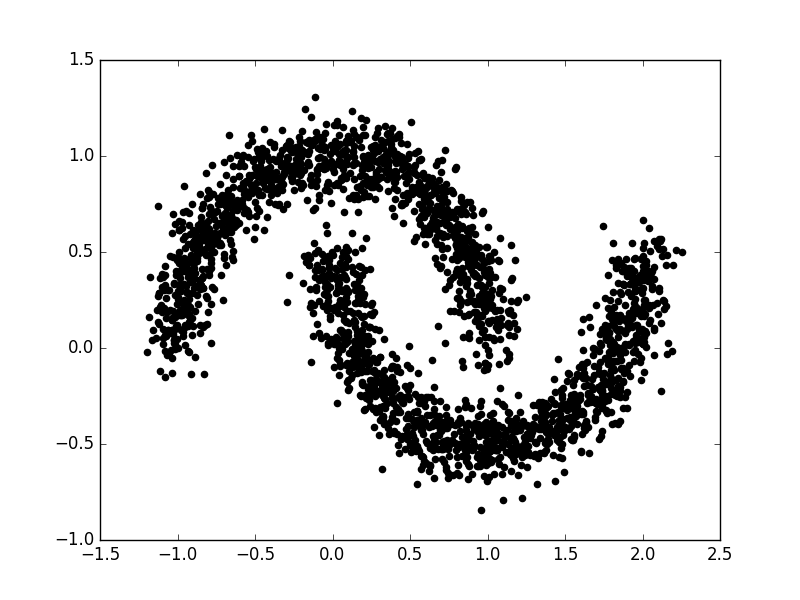
\includegraphics[width=\linewidth]{figuras/initial.png}
	\caption{Conjunto de dados sintético formado por dois grupos.}
	\label{fig:inital}
\end{figure}

\begin{figure}[h!]
	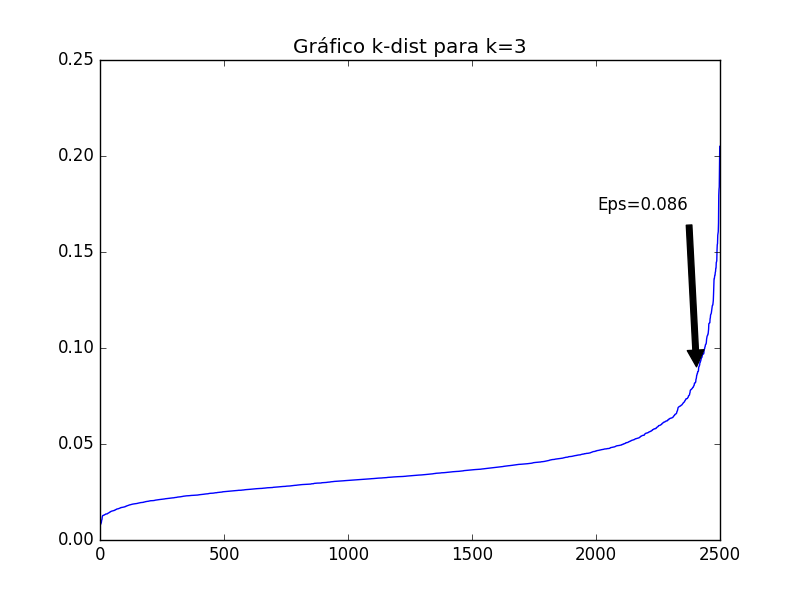
\includegraphics[width=\linewidth]{figuras/k_dist.png}
	\caption{Gráfico \emph{k-dist} do conjunto de dados da figura ~\ref{fig:inital}, onde o crescimento abrupto ocorre para a distância 0.086 aproximadamente.}
	\label{fig:k_dist}
\end{figure}

\begin{figure}[h!]
	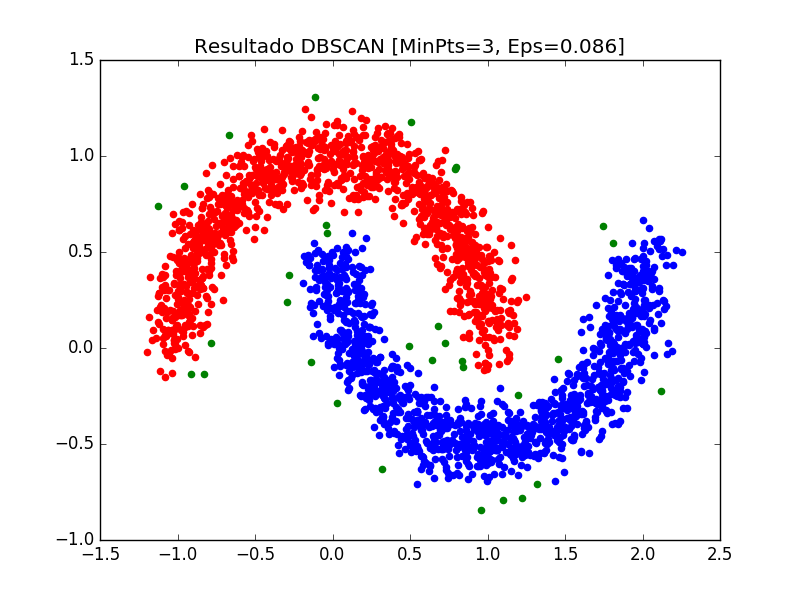
\includegraphics[width=\linewidth]{figuras/result.png}
	\caption{Partição dos dados da figura ~\ref{fig:inital} obtida pelo DBSCAN com \emph{MinPts}=$3$ e \emph{Eps}=$0.086$. O pontos verdes foram considerados \emph{outliers} pelo algoritmo.}
	\label{fig:result}
\end{figure}

Além do método demonstrado, existem outras tentativas para se estimar os melhores valores dos dois parâmetros, de forma automática, como em ~\parencite{DE_DBSCAN}, no qual os valores são obtidos por meio de algoritmos de evolução diferencial. Nesta abordagem, cada indivíduo da população recebe um valor de \textbf{Eps} e \textbf{MinPts}, e uma partição por meio do DBSCAN é obtida para cada indivíduo. A função \emph{fitness} do algoritmo de otimização é dada por índices de validação interna dos grupos, a serem detalhados na seção ~\ref{sec:indice_validacao_interna}, e o algoritmo continua até um critério de parada. Dessa maneira, espera-se alcançar valores de  \textbf{Eps} e \textbf{MinPts} que geram a partição com os melhores índices, que por sua vez refletem em uma melhor partição. Dessa maneira, pode-se afirmar que a abordagem não é muito diferente da estratégia iterativa de obtenção do valor de $k$ dos algoritmos particionais, nos quais os algoritmos têm que ser executados diversas vezes. Já em ~\parencite{OPTICS}, é proposto o algoritmo OPTICS, \emph{Ordering Points to Identify the Clustering Structure}, no qual se faz necessária somente a informação do valor de \textbf{MinPts}, sendo o \textbf{Eps} estimado pelo próprio algoritmo. 

Apesar de no exemplo apresentado a distância euclidiana ter sido utilizada, o DBSCAN pode receber como parâmetro uma matriz de dissimilaridade gerada por qualquer outra dissimilaridade, o que, no contexto de séries temporais, o torna bastante interessante. O custo computacional do DBSCAN é de $\mathcal{O}(n \log n)$.

\section{Índices de validação de agrupamentos}

Após a definição de uma métrica de dissimilaridade, da escolha de um algoritmo de agrupamento, e da realização do agrupamento em si, faz-se necessária a avaliação da partição obtida. Tal avaliação é realizada pelos índices de validação que podem ser divididos em dois grandes grupos, sendo o primeiro formado pelos índice de validação interna enquanto o segundo contém os índices de validação externa. 

Os índices de validação interna são utilizados quando não se dispões de informações externas dos dados, e dessa maneira, ele é obtido apenas pelo resultado do agrupamento e das dissimilaridades entre as instâncias. Por sua vez, os índices de validação externos, utilizam alguma outra informação, além do resultado do agrupamento, no cálculo do índice. Tal informação externa é o resultado esperado do agrupamento, ou seja, os rótulos de cada instância. Uma discussão mais profunda de cada um dos tipos de índices de validação de agrupamentos é realizada a seguir.

\subsection{Índices de validação interna} \label{sec:indice_validacao_interna}

Normalmente, nas tarefas de agrupamento de dados, os índices de validação interna são os mais utilizados, pelo fato de não se possuir \emph{a priori} a rotulação das instâncias. Os índices de validação internos podem ser úteis também para a definição de um valor $k$ que represente o número de grupos, no qual os dados se encontram naturalmente distribuídos. O número pode ser aproximado ao se obter diversas partições para valores iterativos de $k$, e a partição que acarretar no melhor valor do índice de validação interno será a que possui o valor de $k$ recomendado.

Basicamente duas características são mensuradas pelos índices de validação interna: a \textbf{compactação} dos grupos, ou seja, o quão próximas, ou similares, as instâncias contidas em um mesmo grupo são entre si, e a \textbf{separação} dos grupos, ou seja, o quão distantes, ou dissimilares as instâncias de diferentes grupos são entre si. Cada uma das estratégias descritas a seguir calcula e pondera de formas distintas essas duas características para a obtenção do índice de validação dos resultados do agrupamento.

\subsubsection{\emph{Silhouette}}

O silhouette é um índice de validação proposto por ~\parencite{Rousseeuw:1987:SGA:38768.38772} que tenta avaliar o quão compacta, ou quão similar, cada instância se encontra dentro de seu próprio grupo, e, simultaneamente, o quão distante, ou dissimilar, ela é da instância mais próxima, ou mais similar, à ela e que não pertence ao seu mesmo grupo.

Para cada instância $x_i$ do conjunto de dados $X$ contendo $n$ instâncias, agrupada no grupo $\mathcal{C}_k$, devem ser calculados dois valores, sendo o primeiro a média da métrica de dissimilaridade entre $x_i$ e as demais instâncias contidas em $\mathcal{C}_k$, denominado $a$, e o segundo como o valor mínimo dentre todas as dissimilaridades entre $x_i$ e as demais instâncias não contidas em $\mathcal{C}_k$, denominado $b$. O valor de silhouette $S_i$ do ponto $x_i$ é definido como:
\begin{equation}
S_i = \frac{(b-a)}{\max(a,b)}, \mathrm{onde}
\end{equation}

\begin{equation}
a = \frac{1}{n} \sum_{j}^{|\mathcal{C}_k|} dist(x_i,x_j); x_j, x_i \in \mathcal{C}_k,
\end{equation}

\begin{equation}
b =\min(dist(x_i,x_j)); x_i \in \mathcal{C}_k,  x_j \notin \mathcal{C}_k,
\end{equation}
sendo $dist(x_i,x_j)$ o valor da métrica de dissimilaridade entre as instâncias $x_i$ e $x_j$.

Os valores de $S_i$ variam de $-1$ a $1$, sendo o valor de $-1$ geralmente quando a atribuição da instância $x_i$ ao seu grupo é equivocada, e $1$ quando é acertada. Valores próximos de $0$ podem indicar sobreposição de grupos. O valor de silhouette da partição é definido como a média dos valores de cada instância do conjunto de dados:

\begin{equation}
S = \frac{1}{n} \sum_{i}^{n} S_i.
\end{equation}

Valores próximos de $1$ indicam uma boa partição, ao passo que valores próximos de $-1$ indicam uma partição ruim.

\subsubsection{Índice de Dunn}

Proposto por ~\parencite{Dunn}, o índice de Dunn é definido como a razão entre a mínima distância intragrupo e a máxima intergrupo. Sendo assim, dada uma partição com $K$ grupos, sendo $\mathcal{C}_k$ o k-ésimo grupo dessa partição, então $dist_{kk'}$ é definida como a menor distância entre cada uma das  $n_k$ e $n_k'$ instâncias dos grupos $\mathcal{C}_k$ e $\mathcal{C}_k'$ respectivamente:

\begin{equation}
dist_{kk'} = \min_{i=1,...,n_k\\j=1,...,n_{k'}} \text{			} \bigg(dist(x_{i}^{k},x_{j}^{k'})\bigg),
\end{equation}
e $d_{min}$ é a menor destas distâncias:

\begin{equation}
d_{min} = \min_{k \neq k'} dist_{kk'}.
\end{equation}

O diâmetro do grupo $\mathcal{C}_k$, é definido como a maior distância entre os distintos $n_k$ pontos contidos pelo grupo $\mathcal{C}_k$:

\begin{equation}
D_k = \max_{x_i,x_j \in \mathcal{C}_k, x_i \neq x_j} dist(x_i,x_j),
\end{equation}
e finalmente, o maior diâmetro da partição é definido como $d_{max}$:

\begin{equation}
d_{max} = \max_{1\leq k \leq K} D_k.
\end{equation}

O índice \emph{Dunn} é definido pela razão entre $d_{min}$ e $d_{max}$:

\begin{equation}
Dunn = \frac{d_{min}}{d_{max}}
\end{equation}

O índice \emph{Dunn} varia de $[0,\infty)$ e valores menores implicam em partições melhores.

\subsubsection{\emph{Davies-Bouldin Index}}

Proposto em ~\parencite{DBI}, o índice Davies-Bouldin é obtido da seguinte maneira: dada um partição com $K$ grupos e sendo $G_k$ o ponto definido como o ponto mais representativo do k-ésimo grupo, onde por mais representativo entende-se o centróide no espaço euclidiano e o medóide para outras métricas de dissimilaridade, então a  distância média $\delta_k$ entre cada instância e seu ponto mais representativo é definida como:

\begin{equation}
\delta_k = \frac{1}{n_k}\sum_{i}^{n_k} dist(x_i,G_k),
\end{equation}
onde $n_k$ é número de instâncias contidas no k-ésimo grupo e $x_i$ é a i-ésima instância do grupo $k$. Essa métrica de compactação de grupo deve ser calculada para cada uma dos $k$ grupos da partição, e a dispersão entre os grupos é calculada entre cada um dos pares de grupos que formam a partição:

\begin{equation}
\Delta_{kk'} = dist(G_k,G_k').
\end{equation}

Finalmente, o índice Davies-Bouldin é definido como:

\begin{equation}
DBI = \frac{1}{K}\sum_{k=1}^{K} \max_{k \neq k'} \bigg( \frac{\delta_k + \delta_k'}{\Delta_{kk'}}  \bigg).
\end{equation}

O DBI é um índice de validação interna definido em $[0,\infty)$, e quanto maior o seu valor melhor é considerada a partição.


\subsubsection{Índice de Calinski-Harabasz}

Em \parencite{CH} é proposto um índice de validação para a identificação de grupos em um espaço euclidiano. Para tal ele define uma métrica que pondera as variâncias intragrupo WGSS (\emph{within-group sum of sqaure distance }), entendida como a variância da distância entre o centróide de um grupo e as suas instâncias, e a dispersão entre os grupos BGSS (\emph{between group sum of square distances}), entendida como a dispersão entre os centróides de cada grupo e o centróide de todo o conjunto de dados. Os valores obtidos são ponderados em função do número de grupos $k$. Então, o índice de Calinski-Harabasz é definido como

\begin{equation} \label{eq:CH}
CH = \frac{\frac{\text{BGSS}}{k-1}}{\frac{\text{WGSS}}{n-k}},
\end{equation}
sendo
\begin{equation}
BGSS=\sum_i{n_i d^2(c_i,c)}
\end{equation}
e
\begin{equation}
WGSS=\sum_i\sum_{x \in C_i} d^2(x,c_i),
\end{equation}
onde $c_i$ e $c$ são os centróides do i-ésimo grupo e o centróide de todo o conjunto de dados respectivamente, e $d(x_1,x_2)$ é a distância euclidiana entre os pontos $x_1$ e $x_2$.

Apesar de ter sido definido para o espaço euclidiano, os próprios autores em \parencite{CH} fazem menção à possibilidade de extensão do índice a espaços não-euclidianos. Para tal, basta utilizar outros conceitos como o medóide, ao invés do centróide, e a própria distância não-euclidiana entre os medóides e as instâncias ao invés da distância euclidiana entre os centróides e as instâncias.

Uma partição ideal tem alta dispersão entre os grupos (BGSS), e baixa variância intragrupo (WGSS), de forma que pela equação ~\ref{eq:CH} fica evidente que valores grandes de CH são desejados. O índice em questão é definido no intervalo $]0,\infty)$.

%\subsubsection{Índice I}

%O índice I, é definido em \parencite{I} como

%\begin{equation} \label{eq:I}
%\bigg( \frac{1}{k} . \frac{\sum_{x \in X} d(x,c)}{\sum_i\sum_{x \in C_i} d(x,c_i)} . max_{i,j} d(c_i,c_j)\bigg)^p,
%\end{equation}
%onde $k$ é o número de grupos, $C_i$ é o i-ésimo grupo e $c_i$ é o ponto mais representativo do i-ésimo grupo, definido como o centróide para espaços euclidianos e medóide para espaços não-euclidianos. Por sua vez, $p$ é um valor de correção e sugerido igual a $2$.

%Como pode ser visto pela equação ~\ref{eq:I}, o índice é composto por três termos:

%\begin{itemize}
%	\item $\frac{1}{k}$ cuja função é reduzir o índice com o incremento de $k$,
%	\item $\frac{E_1}{E_k}$ onde o termo $E_1$ é constante para determinado conjunto de dados e o termo $E_k$ diminui com o crescimento de $k$ indicando 
%\end{itemize}

%\hl{TODO}

%\subsubsection{Índice de Xie-Beni}
%\hl{TODO}

\subsection{Índices de validação externa}

Em tarefas reais de agrupamento, os índices de validação externa não têm utilidade direta, pois como já dito, em tarefas de agrupamento não se dispõe \emph{a priori} do rótulo das instâncias. Eles são muito úteis para se validar parâmetros e estratégias de agrupamento, ao se obter um valor numérico que faça com que seja possível comparar o resultado obtido  de cada abordagem com o resultado esperado.

Assim, variando-se os algoritmos, métricas, estratégias de pré-processamento e outros parâmetros ou decisões da tarefa de agrupamento de determinado conjunto de dados rotulado, pode-se comparar cada partição obtida com a partição real, ou verdadeira. Ou seja, caso se deseje realizar o agrupamento de dados não rotulados, e não se sabe a melhor estratégia para tal, se, primeiramente,  o agrupamento for feito em uma base de dados que seja, de alguma forma, semelhante à base alvo e a primeira esteja rotulada, então os índices de validação externa podem ser úteis na obtenção de uma estratégia mais adequada para a base não rotulada. %A seguir seguem alguns comentários sobre os principais índices de validação externa.

Existem diversos índices de validação externa tais como o \emph{Adjusted Rand Index} (ARI) ~\parencite{Hubert1985}, \emph{Adjuste Mutual Info } (AMI) ~\parencite{AMI}, \emph{V-measure} ~\parencite{V_measure}, \emph{Variation of Information} (VI) ~\parencite{Meila}, entre outros. Neste trabalho, o índice VI foi especialmente utilizado, pelo fato de, diferentemente dos demais, ser uma métrica no espaço de partições. Dada a sua importância, ele se encontra detalhado na seção seguinte.


\subsubsection{\emph{Variation of Information} - VI} \label{sec:VI}

Proposto em ~\parencite{Meila}, e baseado em técnicas da teoria da informação, o VI mede a quantidade de informação ganha ou perdida ao se mudar da partição $\mathcal{P}$ para a partição $\mathcal{P'}$. O VI possui a propriedade de ser uma métrica de distância no espaço de partições, ou seja, obedece aos quatro axiomas apresentados no início da seção ~\ref{sec:metricas}. Essa propriedade faz com que seja possível, por exemplo, realizar o agrupamento de partições. 

Assim, dada uma partição $\mathcal{P}$ formada por $n$ instâncias divididas em $k$ grupos, onde o k-ésimo grupo contém $n_k$ instâncias, podemos definir uma variável aleatória como a probabilidade de se escolher uma instância do k-ésimo grupo e a entropia da partição como:

\begin{equation}
P(k) = \frac{n_k}{n}\text{ e,}
\end{equation}

\begin{equation}
H(\mathcal{P}) = -\sum_{i}^{k}P(k) \log P(k).
\end{equation}

Sendo $P(k)$ e $P'(k')$ as variáveis aleatórias associadas às partições $\mathcal{P}$ e $\mathcal{P'}$ respectivamente. Então, pode-se definir a probabilidade de uma instância pertencer ao grupo $\mathcal{C}_k$ da partição $\mathcal{P}$ e ao grupo $\mathcal{C'}_{k'}$ da partição $\mathcal{P'}$ como:

\begin{equation}
P(k,k') = \frac{|\mathcal{C}_k\cap \mathcal{C'}_{k'}|}{n},
\end{equation}
e a informação mútua entre as partições $\mathcal{P}$ e $\mathcal{P'}$ como:

\begin{equation}
I(\mathcal{P},\mathcal{P'}) = \sum_{i}^{k} \sum_{i}^{k'} P(k,k') \log \frac{P(k,k')}{P(k)P'(k')}.
\end{equation}

Finalmente, a variação da informação entre as partições $\mathcal{P}$ e $\mathcal{P'}$ pode ser definida como:

\begin{equation}
VI(\mathcal{P},\mathcal{P'}) = H(\mathcal{P}) + H(\mathcal{P'}) - 2I(\mathcal{P},\mathcal{P'}).
\end{equation}
Pelo fato do índice em questão ser uma métrica no espaço de partições, se soubermos a partição esperada, ou verdadeira, de um conjunto de dados, denominada $\mathcal{P}_v$, e possuirmos duas partições de teste $\mathcal{P}_{t1}$ e $\mathcal{P}_{t2}$, a partição de teste que possuir menor VI em relação à partição verdadeira, é considerada uma melhor partição dos dados do que a outra partição de teste. Ou seja,:

\begin{equation}
\begin{cases}
\text{se } VI(\mathcal{P}_v,\mathcal{P}_{t1})  < VI(\mathcal{P}_v,\mathcal{P}_{t2})\text{, então $\mathcal{P}_{t1}$ é melhor, ou mais verossímel, que $\mathcal{P}_{t2}$} ,\\
\text{se } VI(\mathcal{P}_v,\mathcal{P}_{t1})  > VI(\mathcal{P}_v,\mathcal{P}_{t2})\text{, então $\mathcal{P}_{t2}$ é melhor, ou mais verossímel, que $\mathcal{P}_{t1}$},\\
\text{se } VI(\mathcal{P}_v,\mathcal{P}_{t1})  = VI(\mathcal{P}_v,\mathcal{P}_{t2})\text{, então $\mathcal{P}_{t2}$ e $\mathcal{P}_{t1}$ são aproximações equivalentes de $\mathcal{P}_v$}.
\end{cases}
\end{equation}

Tais propriedades fazem com que o índice de variação da informação seja extremamente interessante para se construir um ranking entre diversas variações de estratégias de agrupamento para uma mesma base de dados rotulada. Dessa maneira, o VI será utilizado nos testes teóricos a serem realizados no Capítulo ~\ref{cap:testes_teoricos}.

O valores de VI variam de 0, quando $2I(\mathcal{P},\mathcal{P'})=H(\mathcal{P}) + H(\mathcal{P'})$, o que ocorre somente quando $\mathcal{P}=\mathcal{P'}$, até $H(\mathcal{P}) + H(\mathcal{P'})$, o que ocorre quando $I(\mathcal{P},\mathcal{P'}) =0$. Dessa maneira, é possível que o índice VI seja normalizado, dividindo o valor obtido pelo seu valor máximo, que como mencionado é a soma da entropia de cada partição, confinando-o, assim, no intervalo $[0,1]$. No entanto, quando este procedimento é realizado o índice perde a sua característica de métrica no espaço de partições, como provado em ~\parencite{Meila}.

%\subsubsection{\emph{V-Measure Index}}
%\hl{TODO}

%\subsubsection{\emph{IGT - Index of ground truth}}
%\hl{TODO}

%\subsubsection{\emph{Adjusted Rand Index}}
%\hl{TODO}

\section{Conclusões do Capítulo}

Neste capítulo foram apresentados as diversas escolhas que podem ser feitas em tarefas de agrupamento de séries temporais. Inicialmente, foram apresentadas as possíveis operações a serem realizadas em uma fase de pré-processamento como a normalização dos dados, redução de dimensionalidade ou transformadas para se trabalhar no domínio da frequência. Em seguida, foram apresentadas diversas métricas de dissimilaridades e em seguida as possíveis invariâncias desejadas em tarefas de mineração de dados de séries temporais foram enumeradas e exemplificadas. Por fim, os algoritmos mais comuns utilizados no agrupamento de séries temporais, e as estratégias de avaliação de partições, que são realizados por meio de índices internos e externos, foram discutidas.

Após esta revisão acerca do tema de mineração de dados de séries temporais, e, especificamente no contexto de agrupamento, tornou-se evidente a complexidade do assunto, dado, principalmente, às diversas possibilidades de se realizar a tarefa de agrupamento que surgem a partir das diversas combinações possíveis de pré-processamento, métrica de dissimilaridade, algoritmo de agrupamento e método de avaliação do resultado. A cada combinação dessas escolhas dá-se o o nome de estratégia de agrupamento e, uma vez que tal diversidade de estratégias torna difícil a proposição de uma estratégia de agrupamento genérica, faz-se necessário um estudo detalhado e restrito a um número reduzido de escolhas mais promissoras para avaliar a performance de tais escolhas e a consequente proposição de uma estratégia.

Tal estudo foi realizado e os resultados, comentários e conclusões se encontram no Capítulo seguinte (~\ref{cap:testes_teoricos}).
